%%% Работа с русским языком
\usepackage{cmap}					% поиск в PDF
\usepackage[T2A]{fontenc}			% кодировка
\usepackage[utf8]{inputenc}			% кодировка исходного текста
\usepackage[english,russian]{babel}	% локализация и переносы
\usepackage{indentfirst}
\frenchspacing

\usepackage{subfigure}

%%% Дополнительная работа с математикой
\usepackage{amsmath,amsfonts,amssymb,amsthm,mathtools} % AMS
\usepackage{icomma} % "Умная" запятая: $0,2$ --- число, $0, 2$ --- перечисление

%%% Работа с картинками
\usepackage{graphicx}  % Для вставки рисунков
\usepackage{wrapfig} % Обтекание рисунков текстом
\usepackage{subfigure}

%%% Работа с таблицами
\usepackage{array,tabularx,tabulary,booktabs} % Дополнительная работа с таблицами
\usepackage{longtable}  % Длинные таблицы
\usepackage{multirow} % Слияние строк в таблице

%%% Программирование
\usepackage{etoolbox} % логические операторы


\usepackage{setspace} % Интерлиньяж
%\onehalfspacing % Интерлиньяж 1.5
%\doublespacing % Интерлиньяж 2
%\singlespacing % Интерлиньяж 1

\usepackage{lastpage} % Узнать, сколько всего страниц в документе.

\usepackage{soul} % Модификаторы начертания

\usepackage{tikz} % Работа с графикой
\usepackage{pgfplots}
\usepackage{pgfplotstable}

\renewcommand{\phi}{\varphi}
\renewcommand{\epsilon}{\varepsilon}
\usepackage[justification=centering, font=footnotesize]{caption}
\setbeamertemplate{caption}[numbered]

\newcommand{\delayV}[1]{\overset{\leftarrow}{\textbf{x}}_{#1}}
\newcommand{\delayM}[1]{\overset{\leftarrow}{\mathbf{X}}_{#1}}

\usepackage{grffile}
%\usepackage{graphicx}

\setlength{\parskip}{0.1cm}

\author{Сёмкин Кирилл \\ \medskip {\footnotesize Московский Физико-Технический Институт}}
\date{2024}
\title{Тензорная декомпозиция и прогноз для набора временных рядов}

\begin{document}
	
	\begin{frame}[c]
		\titlepage
	\end{frame}

	\begin{frame}{Мотивация}
		
		\begin{alertblock}{Проблема}
			Известные модели многомерных временных рядов (e.g. RNN, VAR) не позволяют строить их аддитивные декомпозиции. Методы разложения одномерных сигналов (e.g. Trend-Cycle Estimation, Seasonal Adjustment Methods) не учитывают взаимозависимость рядов.
		\end{alertblock}
		
		\begin{figure}[h]
			\centering
			
			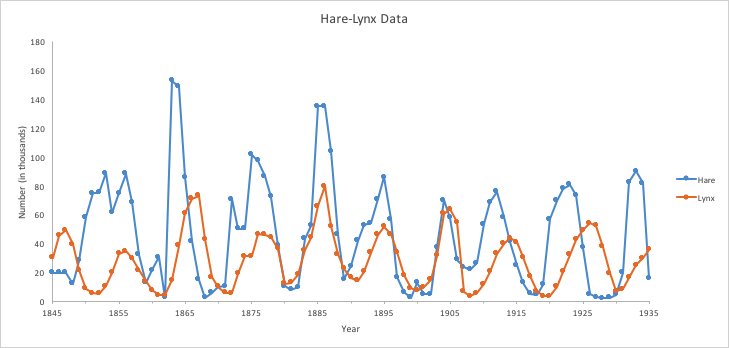
\includegraphics[width=0.69\textheight, keepaspectratio]{img/prey_predetor_graph}
			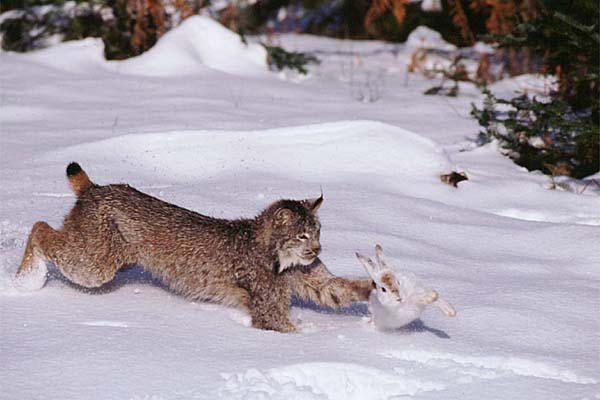
\includegraphics[width=0.28\textheight, keepaspectratio]{img/hare-lynx.jpg}
			
			\caption{График количества особей хищников и травоядных от времени}
			
		\end{figure}
		
	\end{frame}
	
	\begin{frame}{Цель исследования}
		
		Предложить метод, позволяющий выделить общую для набора сигналов структуру. На её основании произвести разложение каждого сигнала на компоненты. Найти способ построения прогноза.
		
		\begin{exampleblock}{Решение}
			\textbf{tSSA} = модель собственного пространства сигнала + тензорное представление данных + CPD
		\end{exampleblock}
		
		Данный подход опирается на гипотезу порождения динамической системой и является расширением метода SSA.
		
	\end{frame}
	
	\begin{frame}{Постановка задачи}
		
		\emph{Динамическая система} в дискретном времени:
		
		\begin{equation*}
			\begin{cases}
				\textbf{y}(t + 1) = f(\textbf{y}(t)), \ t \in \mathbb{N} \\
				\textbf{y}(0) = \textbf{y}_0
			\end{cases}
		\end{equation*}
		
		$ \textbf{y} \in X $, где $ X $ --- гладкое многообразие большой размерности. 
		
		Конкретная траектория этой системы \emph{порождает} наблюдаемые ряды через некое многомерное отображение $ \boldsymbol{\phi}: X \to \mathbb{R}^m $:
		
		\begin{equation*}
			\boldsymbol{\phi}(\textbf{y}(t)) = \textbf{x}_t \Leftrightarrow \begin{cases}
				\phi_1(\textbf{y}(t)) = x_1(t) \\
				\ldots \\
				\phi_m(\textbf{y}(t)) = x_m(t) \\
			\end{cases}
		\end{equation*}
		
	\end{frame}
	
	\begin{frame}{Постановка задачи}
		
		Выдвигается гипотеза, что траектории $ \textbf{y}(t) $ лежат в многообразии $ M \subset X $ размерности  меньшей, чем у $ X $. Ставится задача поиска вложения (embedding) $ M $ в $ \mathbb{R}^{L} $ для некоторого $ L $ и нахождения базиса в образе этого вложения.
		
		\begin{figure}[h]
			\centering
			
			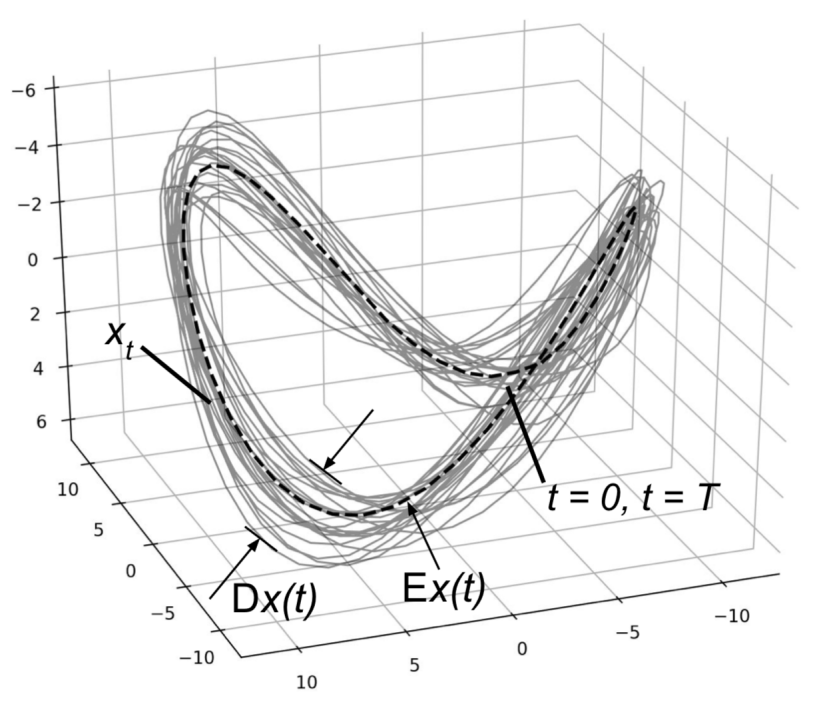
\includegraphics[width=0.6\textheight, keepaspectratio]{img/dynamic_system_example.png}
			\caption{Динамическая система собственной размерности < 3}
			
		\end{figure}
		
	\end{frame}
	
	\begin{frame}{Поиск решения}
		
		\begin{theorem}[Такенс]
			Искомое вложение даётся построением соответствующего вектора задержки 
			
			\begin{equation*}
				\textbf{y}(t) \xrightarrow{emb} \begin{pmatrix}
					\boldsymbol{\phi} \circ f^{t - L + 1}(\textbf{y}(t)) \\
					\vdots \\
					\boldsymbol{\phi} \circ f(\textbf{y}(t)) \\
					\boldsymbol{\phi} \circ \textbf{y}(t)
				\end{pmatrix} = \begin{pmatrix}
					x(t - L + 1) \\
					\vdots \\
					x(t - 1) \\
					x(t)
				\end{pmatrix} = \delayV{t} \in \mathbb{R}^L
			\end{equation*}
			
		\end{theorem}
		
		Полученное пространство вложения $ \text{Lin}(\{\delayV{t}\}) $ и есть \emph{собственное пространство сигнала} $ x(t) $.
		
		C помощью разложения \emph{траекторной матрицы} $ \mathbf{H}_x = [ \delayV{1} \ldots  \delayV{N - L + 1}]. $ выделяем в нём базис. Далее можем декомпозировать и строить прогноз (SSA). 
	
	\end{frame}
	
	\begin{frame}{Метод tSSA}
		
		В случае нескольких рядов упакуем их вектора задержек в \emph{матрицы задержек} $ ( \delayV{1_t} \ldots \delayV{m_t} ) := \delayM{t} $. Состыкуем их в \emph{траекторный тензор} $ \textbf{T} $.
		
		\begin{figure}[h]
			\centering
			\subfigure{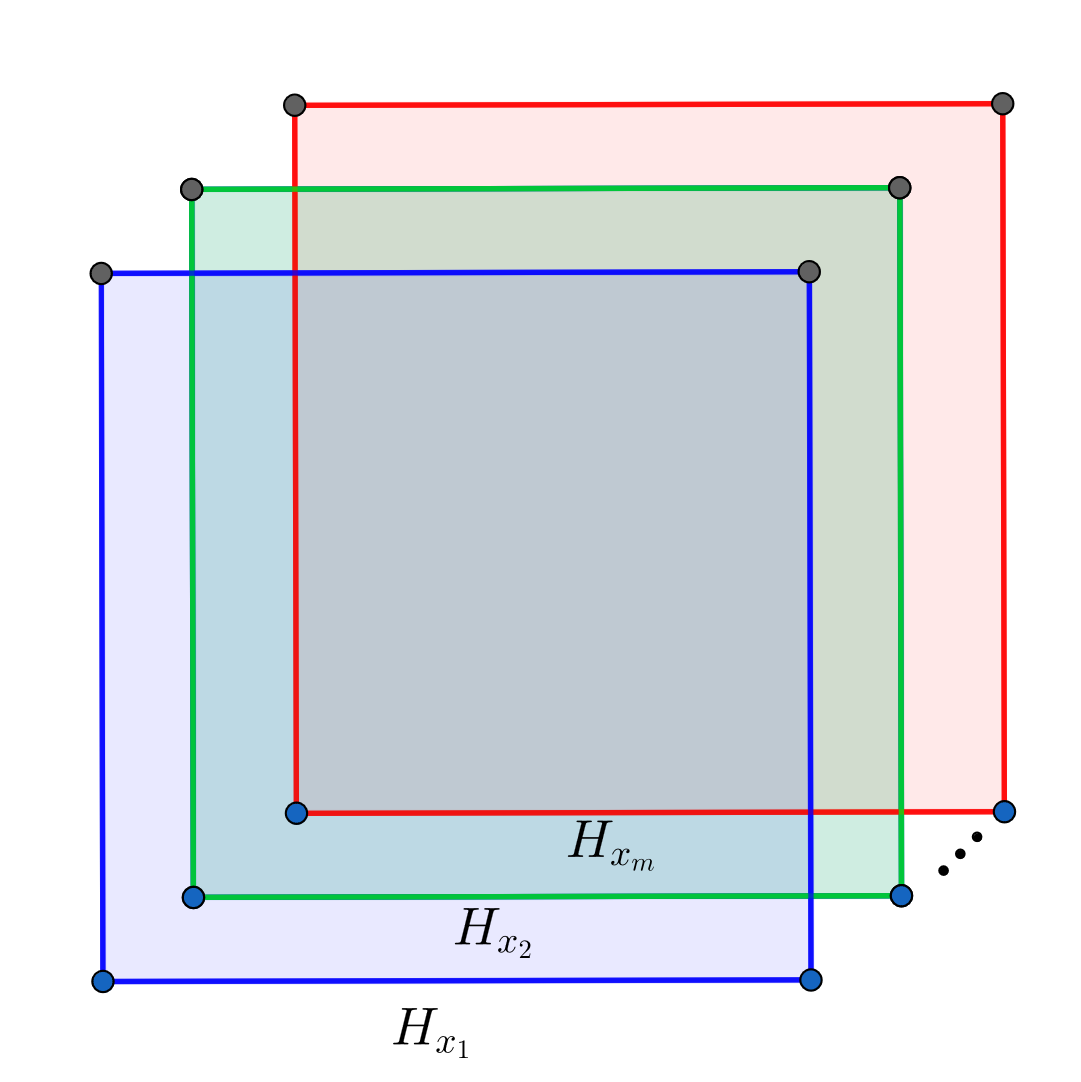
\includegraphics[width=0.4\textwidth, keepaspectratio]{img/Trajectory_Tensor_1}}
			\subfigure{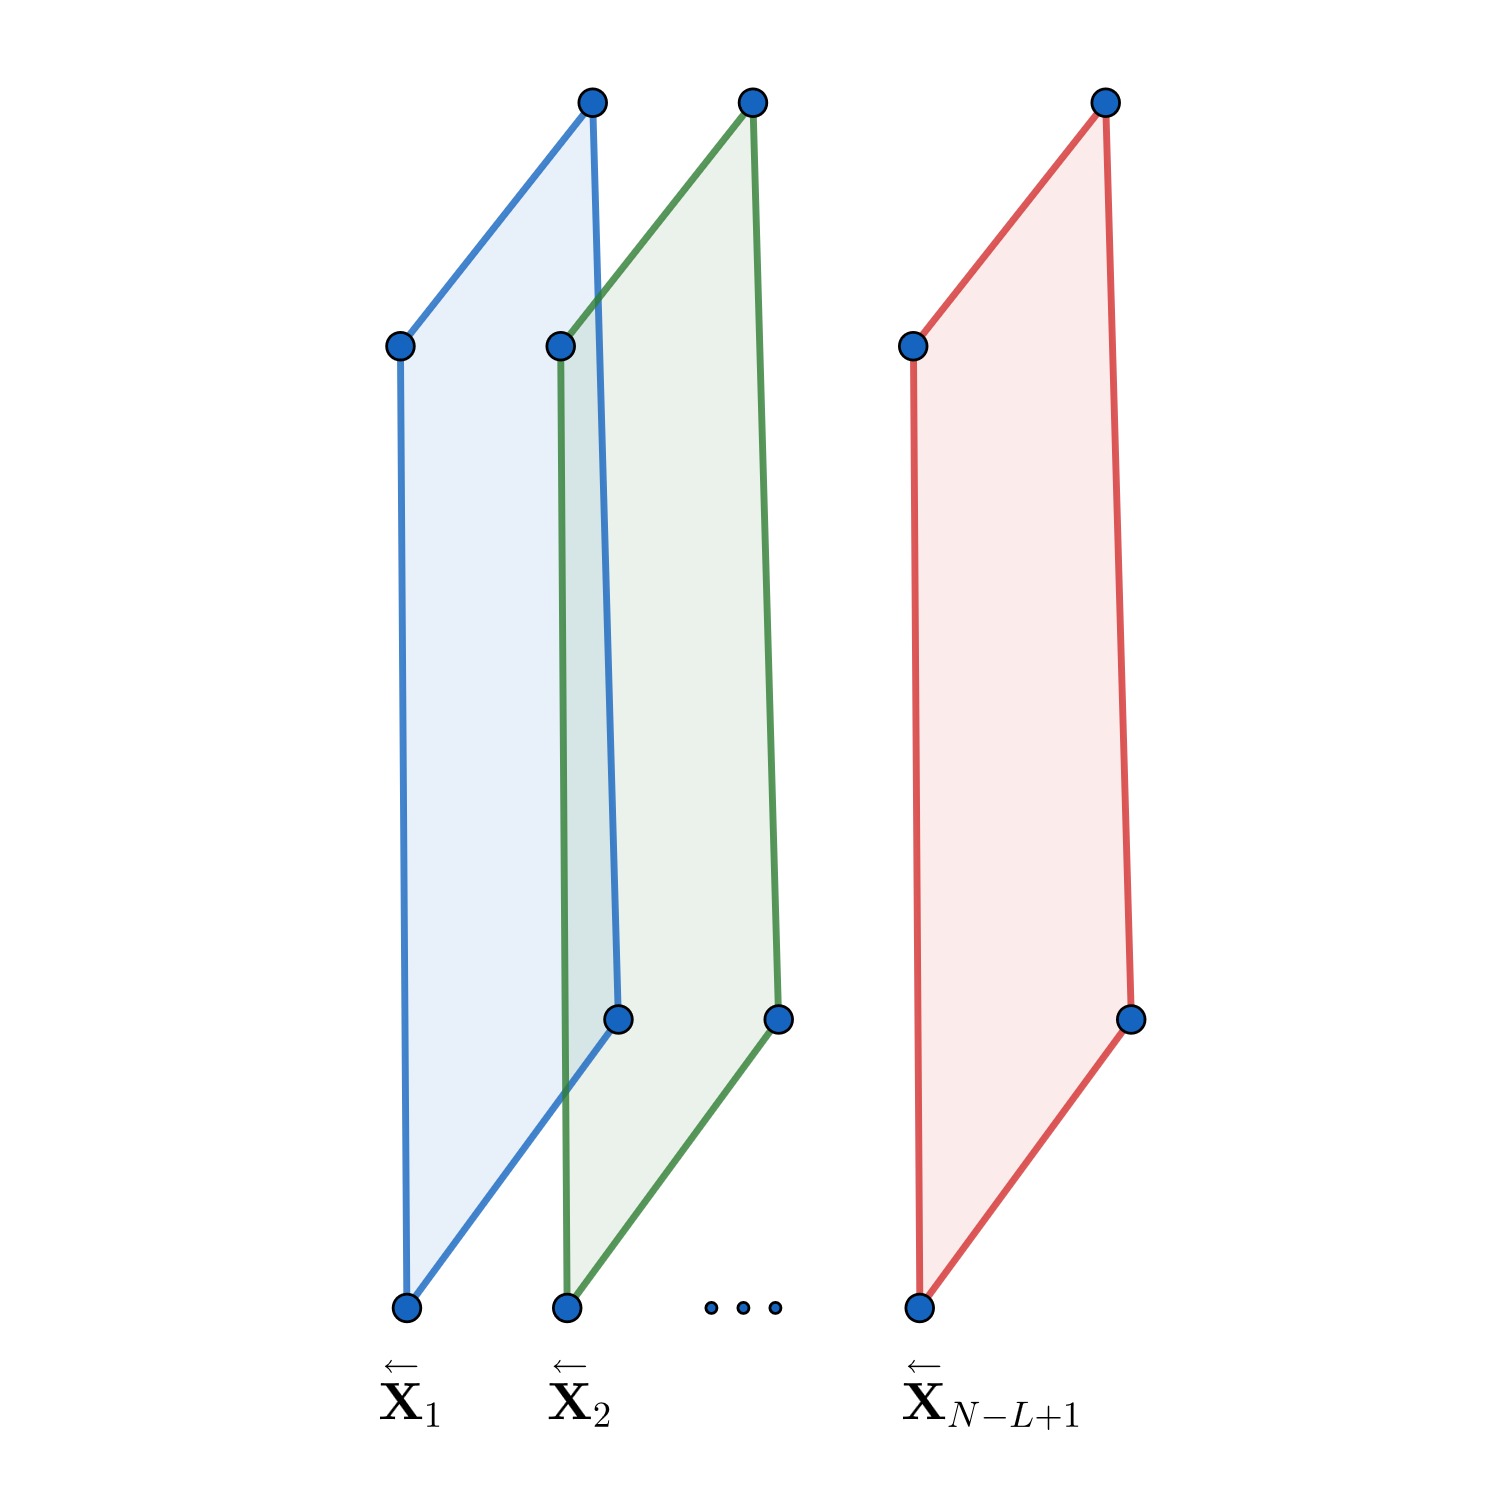
\includegraphics[width=0.4\textwidth, keepaspectratio]{img/Trajectory_Tensor_2}}
			
			\caption{Два вида на $ \textbf{T} $. Слева --- в виде набора траекторных матриц сигналов. Справа --- в виде набора матриц задержки.}\label{pic:traj_tensor}
		\end{figure}
		
	\end{frame}
	
	\begin{frame}{Метод tSSA}
		
		Применим \textit{CPD-разложение} к траекторному тензору и рассмотрим его вид для каждого сечения по третьему измерению:
		
		\begin{equation}\label{eq:tSSA_decomp}
			\textbf{T} = \sum\limits_{i = 1}^{r} \mathbf{a}_i \otimes \mathbf{b}_i \otimes \mathbf{c}_i \Leftrightarrow \begin{cases}
				\mathbf{H}_{x_1} = \sum\limits^{r} \boldsymbol{\sigma}_{x_1}(i) \cdot \mathbf{a}_i  \mathbf{b}_i^{\mathsf{T}}  \\
				\mathbf{H}_{x_2} = \sum\limits^{r} \boldsymbol{\sigma}_{x_2}(i) \cdot \mathbf{a}_i  \mathbf{b}_i^{\mathsf{T}} \\
				\ldots \\
				\mathbf{H}_{x_m} = \sum\limits^{r} \boldsymbol{\sigma}_{x_m}(i) \cdot \mathbf{a}_i  \mathbf{b}_i^{\mathsf{T}} 
			\end{cases}
		\end{equation}
		
		Получили разложение траекторных матриц сигналов по \emph{общему базису}, что выражает предположение взаимосвязанности рядов.
		
	\end{frame}
	
	\begin{frame}{Декомпозиция сигналов}
		
		Для получения декомпозиции факторы разложения $ \mathbf{H}_{x_k} $ разбиваем на группы и \emph{ганкелизуем} --- усредняем матрицы по антидиагоналям.
		
		\begin{multline*}\label{eq:decomp_method_ideal}
			\mathbf{H}_{x_k} = \sum\limits_{i = 1}^{r} \boldsymbol{\sigma}_{x_k}(i) \cdot \mathbf{a}_i  \mathbf{b}_i^{\mathsf{T}} = \sum\limits_{i \in \mathbb{I}_1} \boldsymbol{\sigma}_{x_k}(i) \cdot \mathbf{a}_i  \mathbf{b}_i^{\mathsf{T}} + \ldots + \sum\limits_{i \in \mathbb{I}_s} \boldsymbol{\sigma}_{x_k}(i) \cdot \mathbf{a}_i  \mathbf{b}_i^{\mathsf{T}} = \\ = C_1 + \ldots + C_s = \text{Hankel}(C_1) + \ldots + \text{Hankel}(C_s)  \Leftrightarrow x_k(t) = c_1(t) + \ldots c_s(t)
		\end{multline*}
		
		\begin{alertblock}{Проблема}
			Хочется группировать факторы так, что каждая матрица $ C_i $ была как можно более 'ганкелевой'.
			
			Мера 'ганкелевости' --- \emph{невязка ганкелизации}:
			
			\[
				\text{r}(\mathbf{H}) = \lVert \mathbf{H} - \text{Hankel}(\mathbf{H}) \rVert_{F}^2
			\]
		\end{alertblock}
		
	\end{frame}
	
	\begin{frame}{Декомпозиция сигналов}
		
		Будем искать разбиение факторов, наилучшее в плане средней ганкелевой невязки: $ \frac{1}{s} \sum\limits_{j = 1}^s \text{r}(C_s) \to \min $.
		
		Полученная задача дискретной оптимизации не имеет быстрого алгоритма поиска решения. В работе предложена эвристическая процедура на основе дихотомического разделения групп.
		
		\begin{figure}[h!]
			\centering
			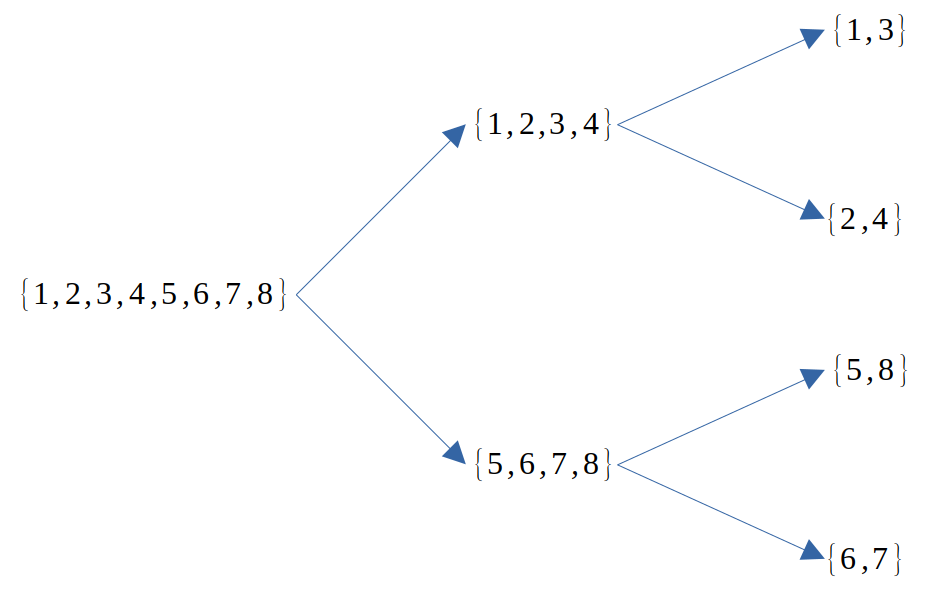
\includegraphics[width=0.45\textwidth, keepaspectratio]{../../figs/dichotomy_drawings/factors.png}    
			$ \mathrel{\raisebox{1.4cm}{$\Leftrightarrow$}} $
			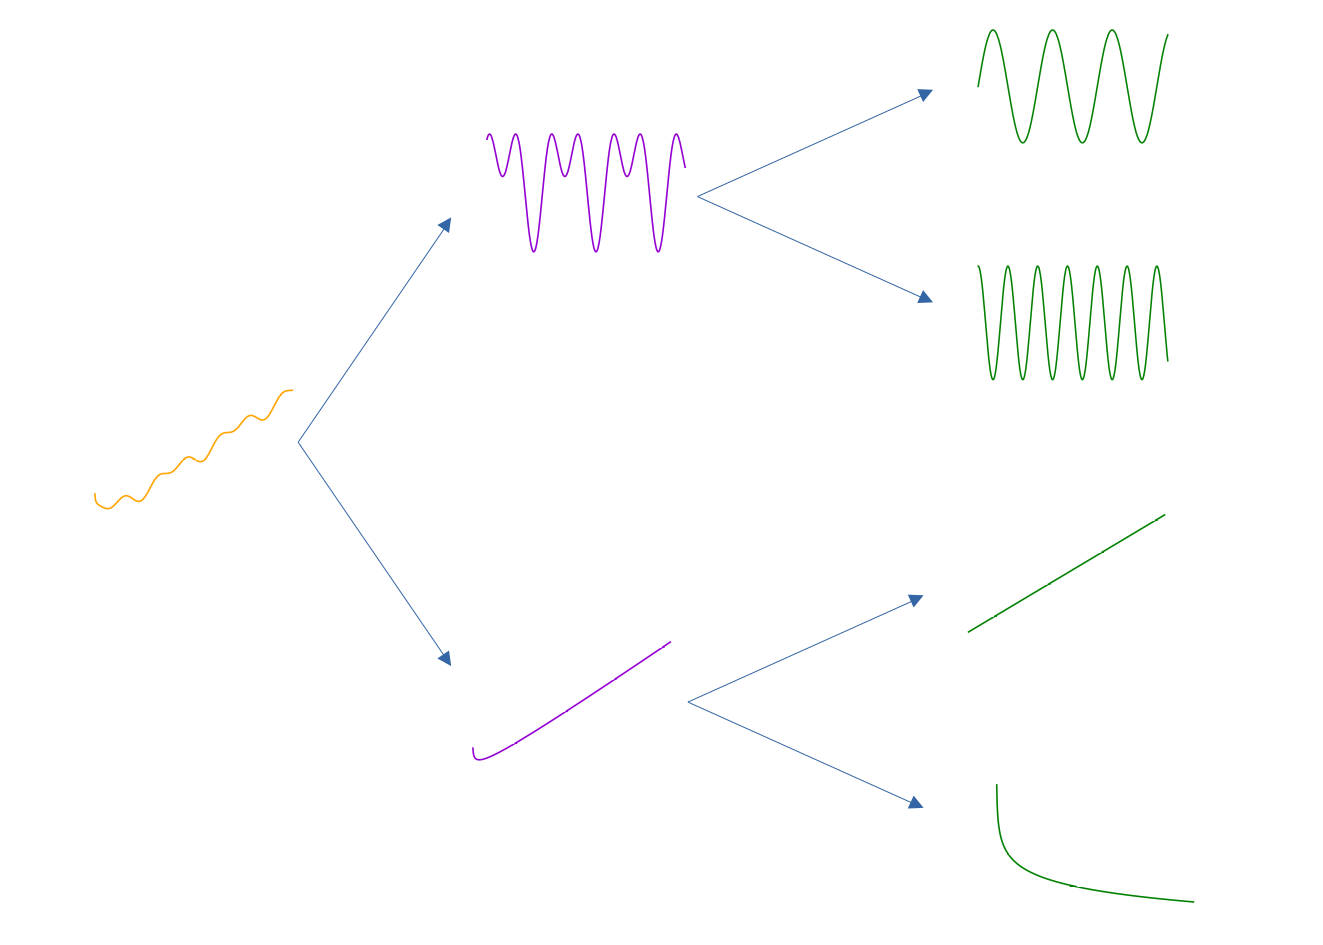
\includegraphics[width=0.45\textwidth, keepaspectratio]{../../figs/dichotomy_drawings/signals.png}	
			
			\caption{Пример рекурсивного разбиения факторов (в виде индексов) на 4 группы и соответствующая декомпозиция сигнала.}\label{pic:decomp_conception}
		\end{figure}
		
	\end{frame}
	
	\begin{frame}{Прогнозирование}
		
		Базис в пространстве векторов задержек сигнала даётся как $ \text{Lin}(\{\mathbf{a}_i\}) \Leftrightarrow A = [\mathbf{a}_1 \ldots \mathbf{a}_r] $. 
		
		Прогноз на один шаг вперёд сводится к решению частично неизвестной СЛАУ:
		
		\begin{gather*}\label{eq:main_pred_for_A}
			\delayV{N + 1} = A \boldsymbol{\lambda} \Leftrightarrow \begin{cases}
				\mathbf{x}_{kn} = A_{kn} \boldsymbol{\lambda}  \\
				x(N + 1) = \mathbf{a}_{pr}^{\mathsf{T}} \boldsymbol{\lambda}
			\end{cases}, \text{ где } \\
			A = \left( \dfrac{A_{kn}}{\mathbf{a}_{pr}^{\mathsf{T}}} \right) \nonumber \\
			\delayV{N + 1} = (\mathbf{x}_{kn}, \  x(N + 1))^{\mathsf{T}} \nonumber
		\end{gather*}
		
		Из-за переопределённости системы, решение выражается в смысле наименьших квадратов:
		
		\begin{equation*}
			x(N + 1) = \mathbf{a}_{pr}^{\mathsf{T}} (A_{kn}^T A_{kn})^{-1} A_{kn}^T \mathbf{x}_{kn}
		\end{equation*}
		
		% TODO: сказать здесь о авторегрессии
		
	\end{frame}
	
	\begin{frame}{Эксперимент}
		
		Цель: 
		
		\begin{itemize}
			\item сравнить качество разложения набора сигналов по \emph{невязке ганкелизации} с методом mSSA. 
			\item сравнить качество построенного прогноза по метрикам \emph{MSE}, \emph{MAPE} с моделями RNN, VAR, mSSA
		\end{itemize}
		
		Рассматриваемые данные:
		
		 \begin{itemize}
		 	\item план выработки электричества на день и его цена производства на МВт
		 	\item погодные условия в Берлине (температура, осадки, атмосферное давление)
		 \end{itemize}
		
	\end{frame}
	
	\begin{frame}{Электричество. Декомпозиция}
		
		\begin{figure}[h]
			\centering
			
			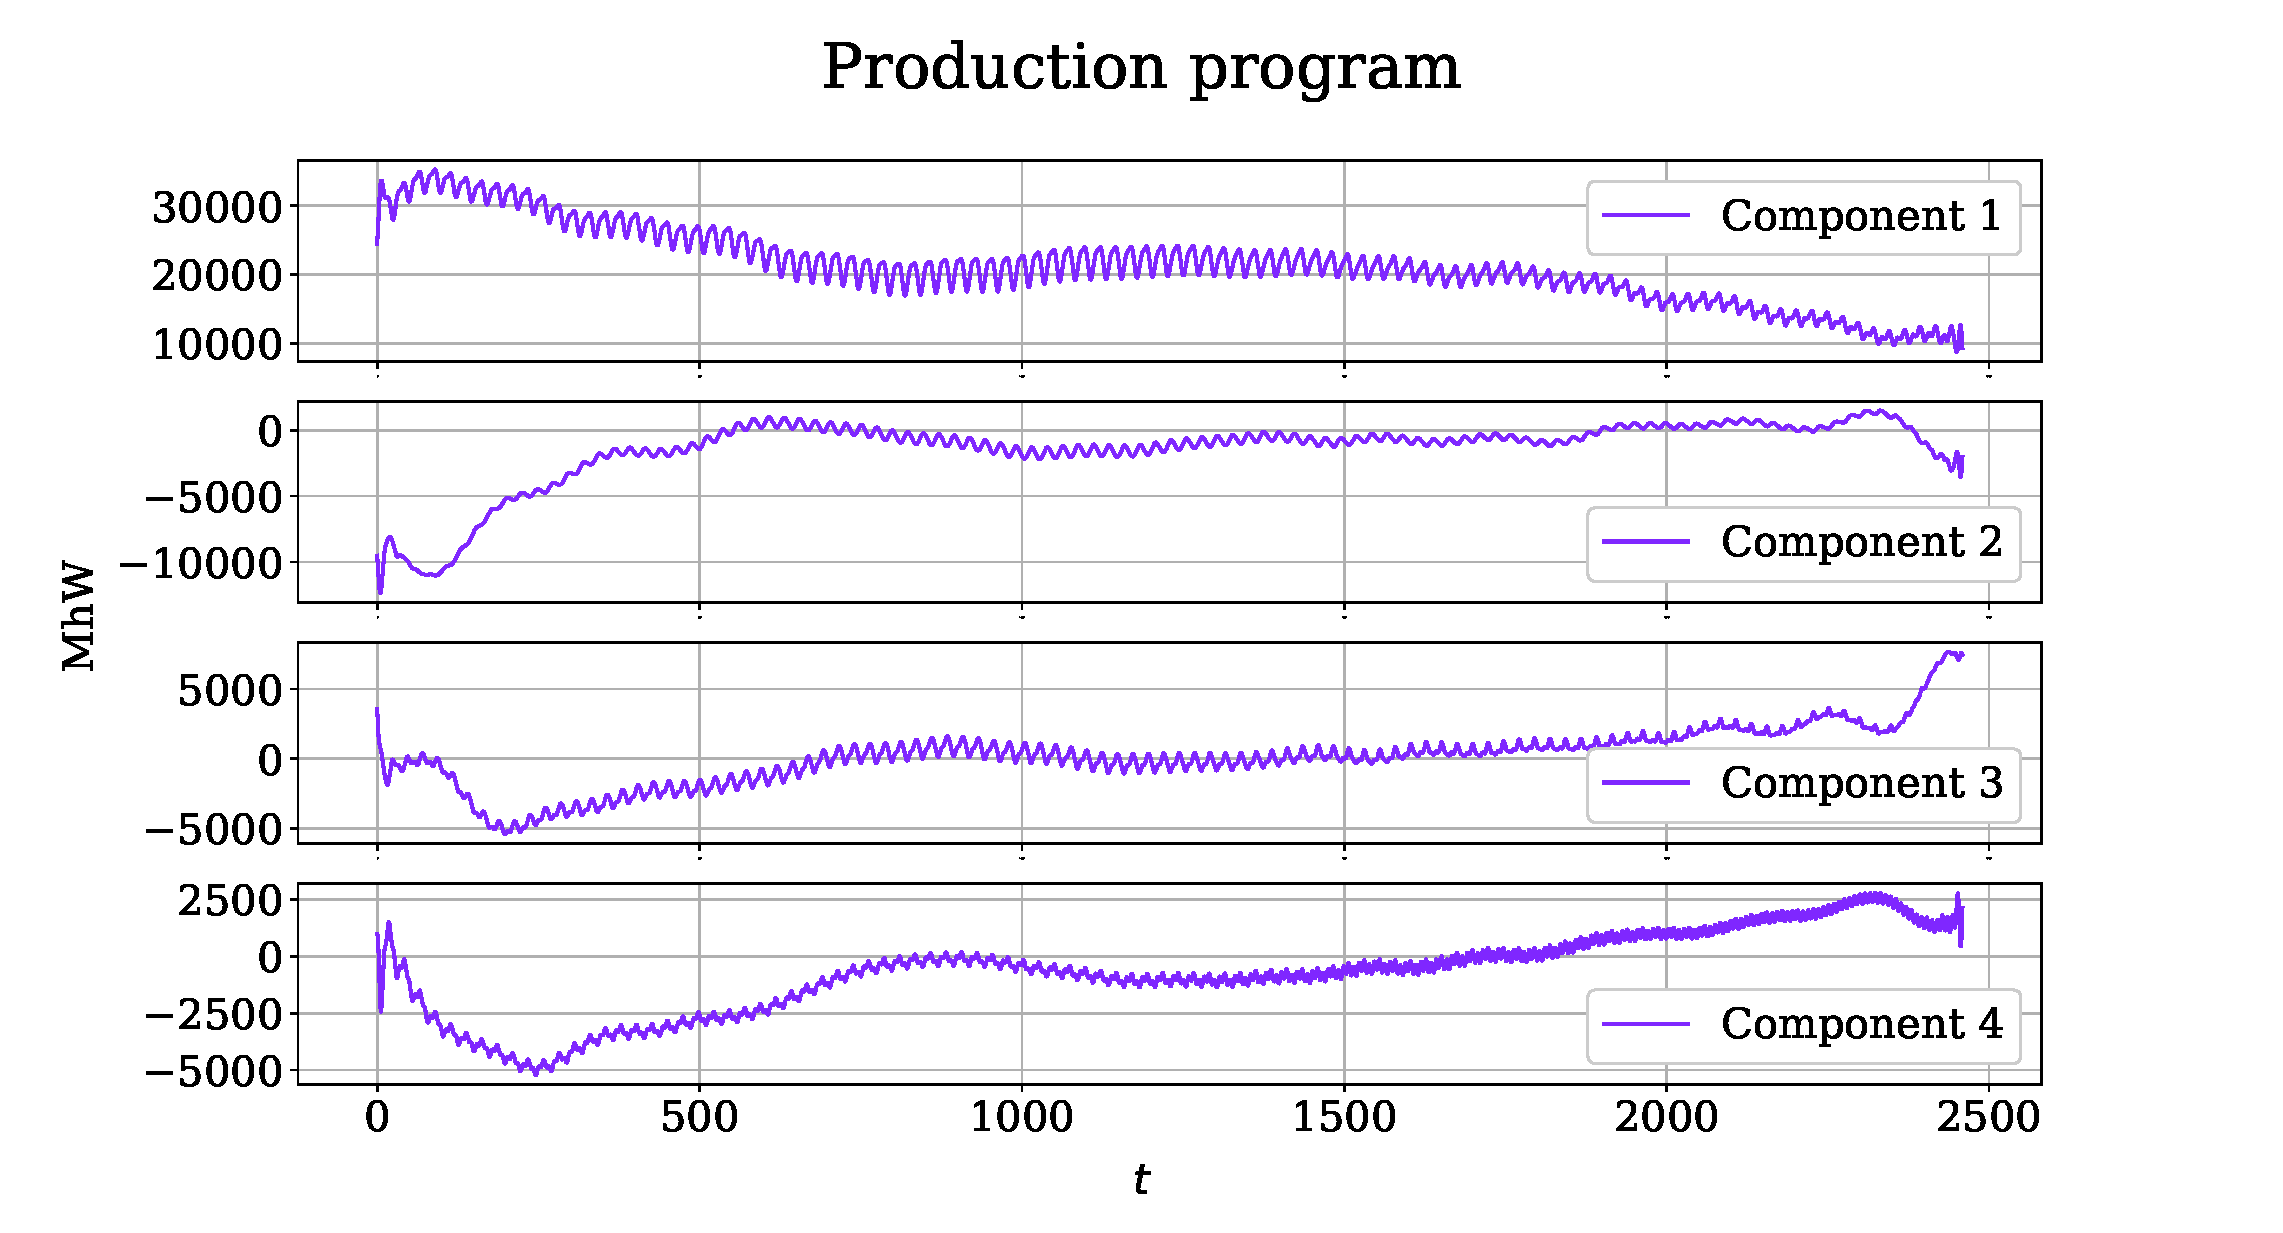
\includegraphics[width=0.49\textwidth, keepaspectratio]{img/electricity/tssa/decomposition/Production_program.eps} 
			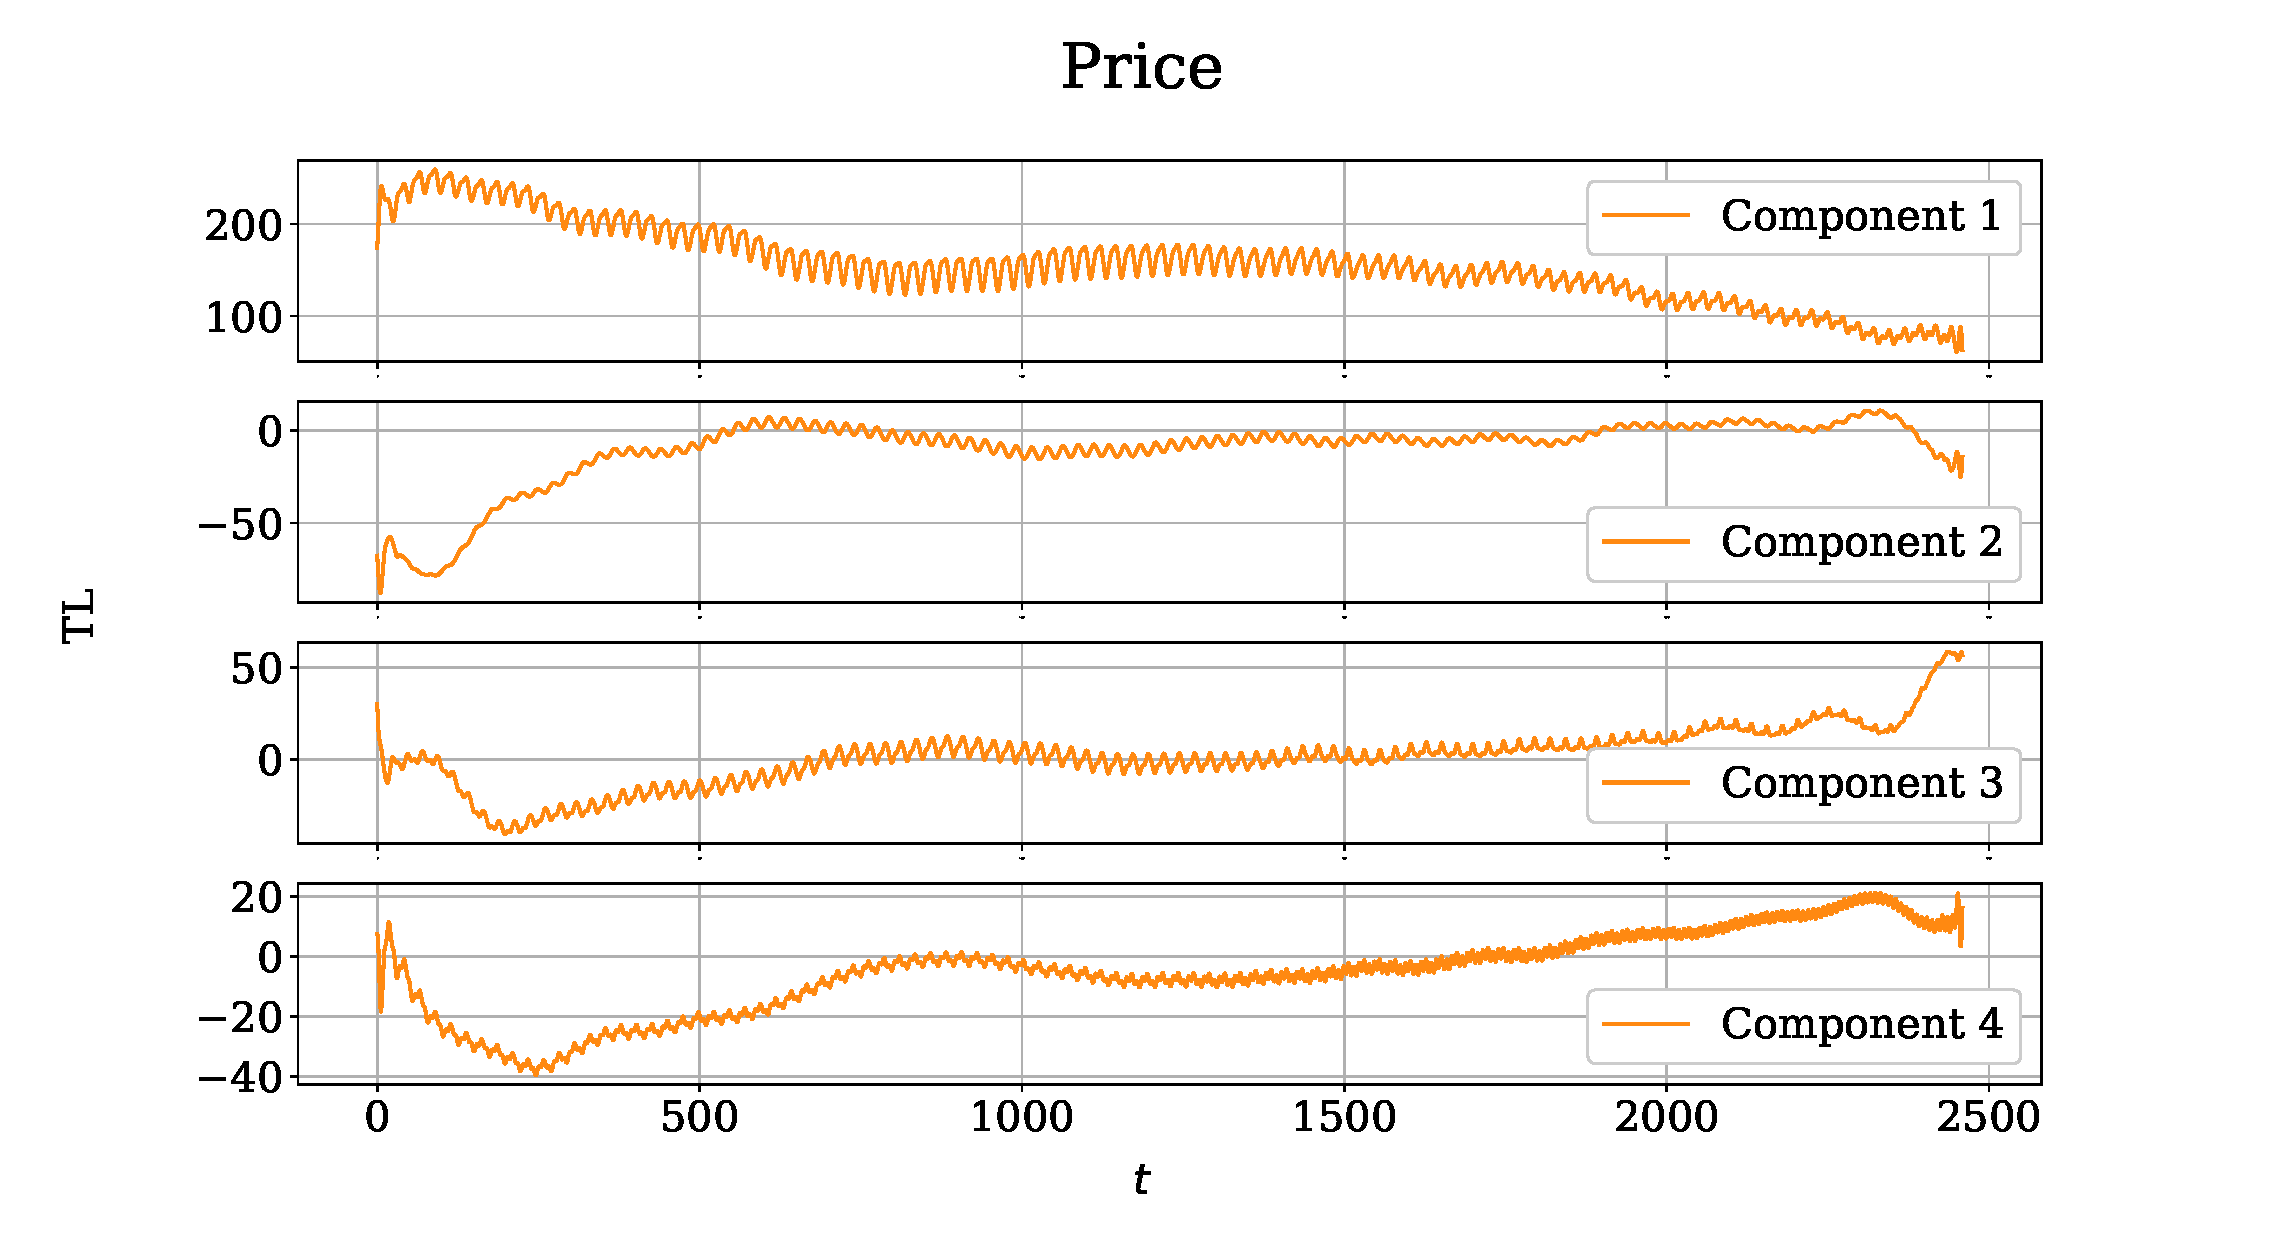
\includegraphics[width=0.49\textwidth, keepaspectratio]{img/electricity/tssa/decomposition/Price.eps}    
			
			\caption{Декомпозия методом tSSA на 4 компоненты через дихотомию. Вид компонент для сигналов идентичный. Наблюдается основной тренд убывания, и три тренда на возрастание. Шумовую часть метод не извлёк.}
		\end{figure}
		
	\end{frame}
	
	\begin{frame}{Электричество. Декомпозиция}
		\begin{figure}[h]
			\centering
			
			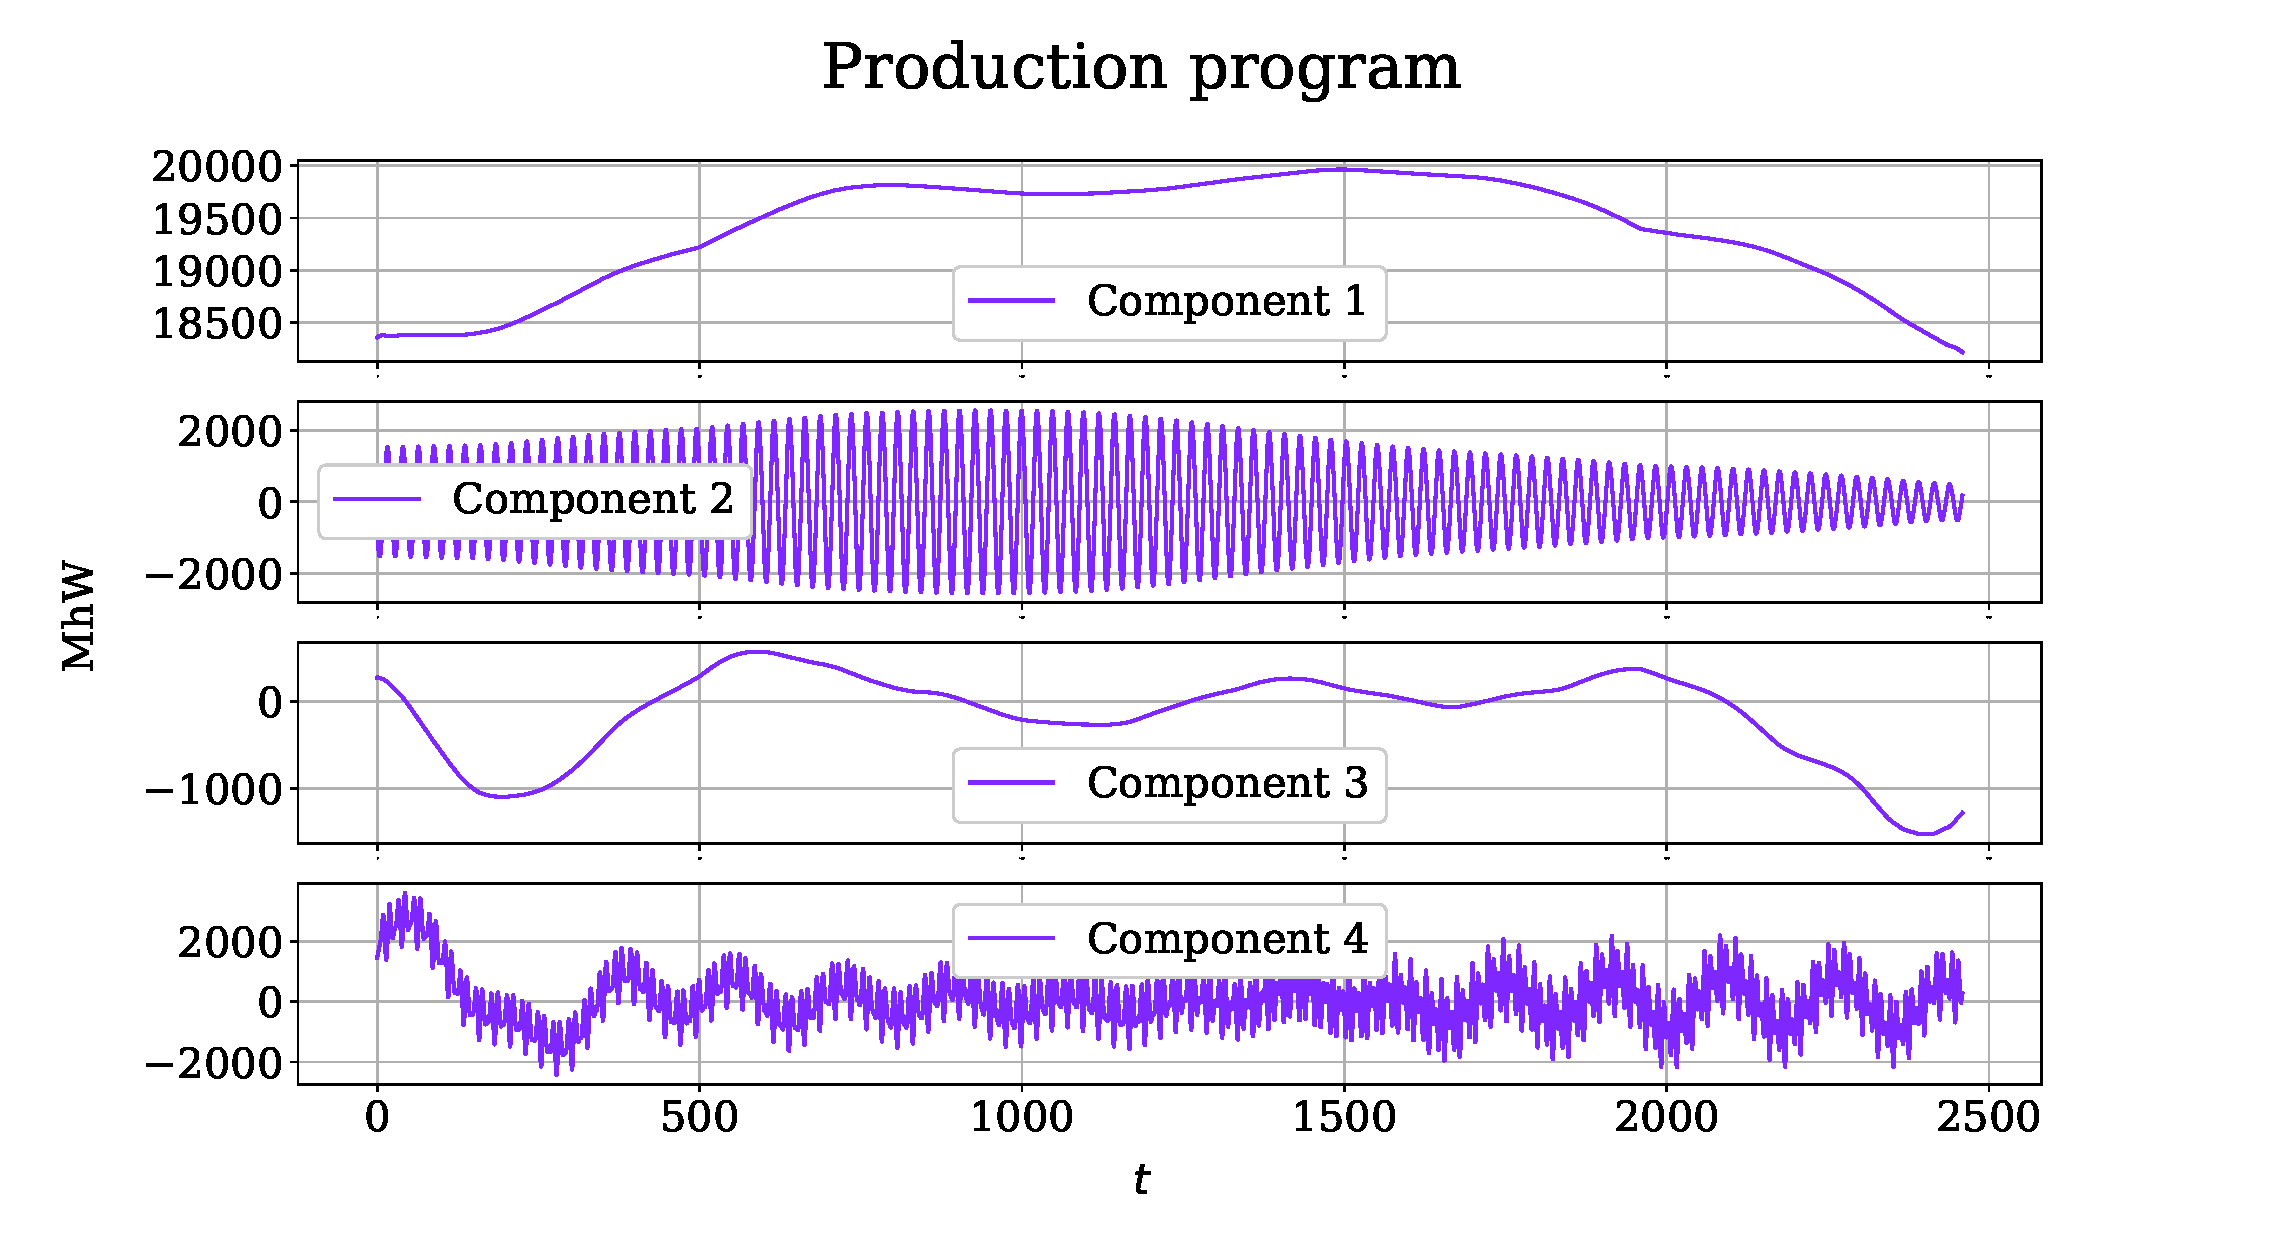
\includegraphics[width=0.49\textwidth, keepaspectratio]{img/electricity/mssa/decomposition/Production_program.eps} 
			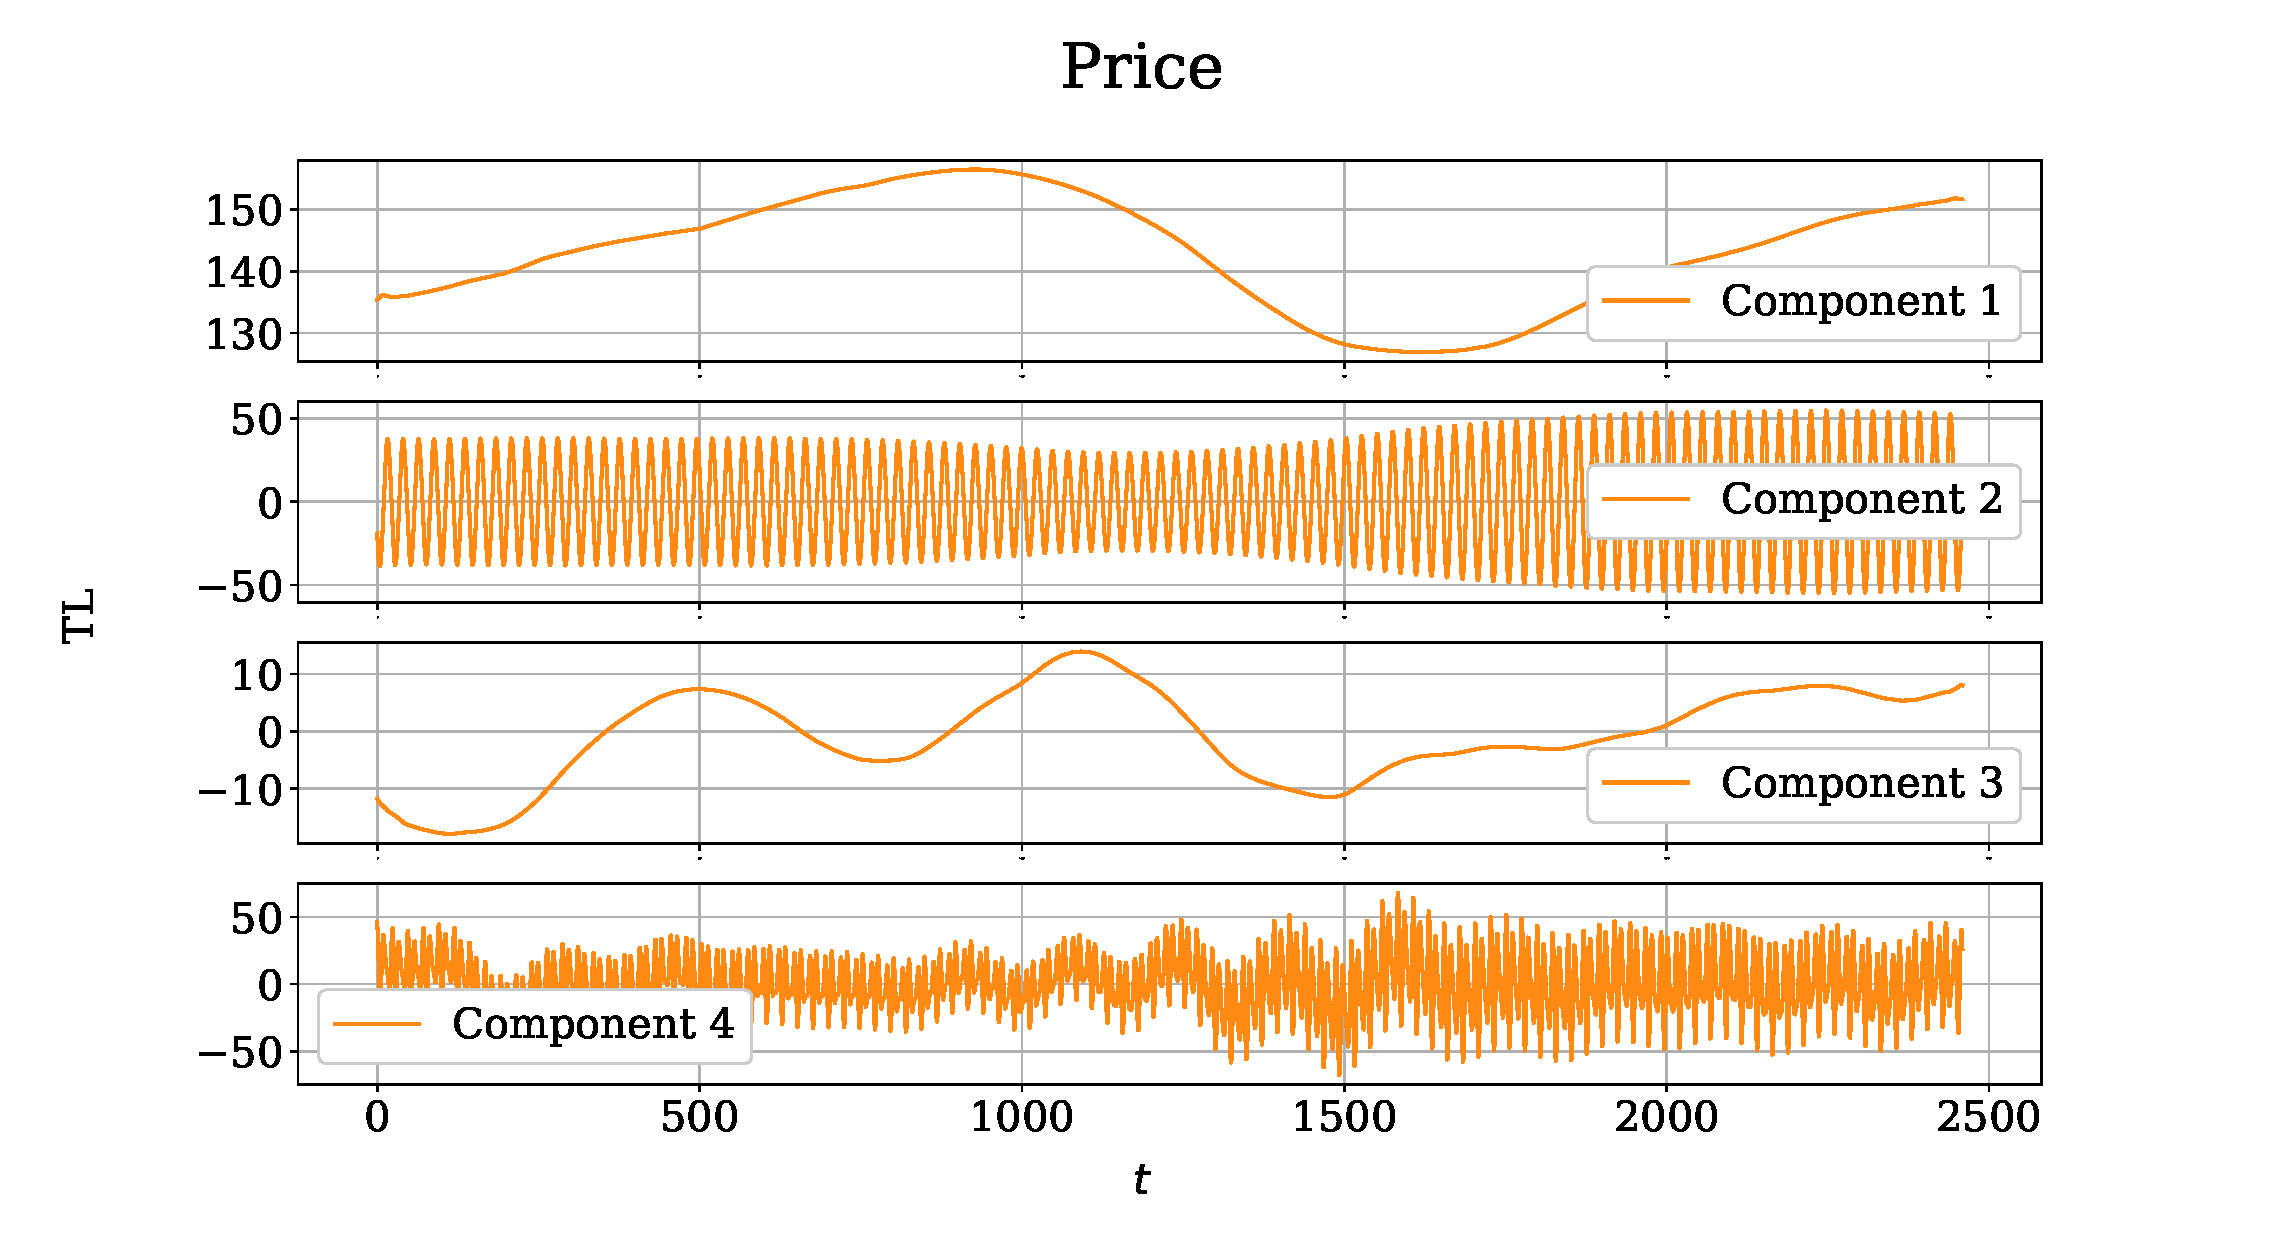
\includegraphics[width=0.49\textwidth, keepaspectratio]{img/electricity/mssa/decomposition/Price.eps}    
			
			\caption{Декомпозия методом mSSA на 4 компоненты подбором групп на основе близости сингулярных чисел. Полученные разложения имеют различный вид для сигналов. Выделены основные тренды и три низкоамплитудных осциллирующих сигнала. Последняя компонента содержит в себе шум, остальные от него очищены.}
		\end{figure}
	\end{frame}
	
	\begin{frame}{Электричество. Прогноз}
		
		\begin{columns}
			
			\column{0.5\textwidth}
			
			\begin{figure}[h]
				\centering
				
				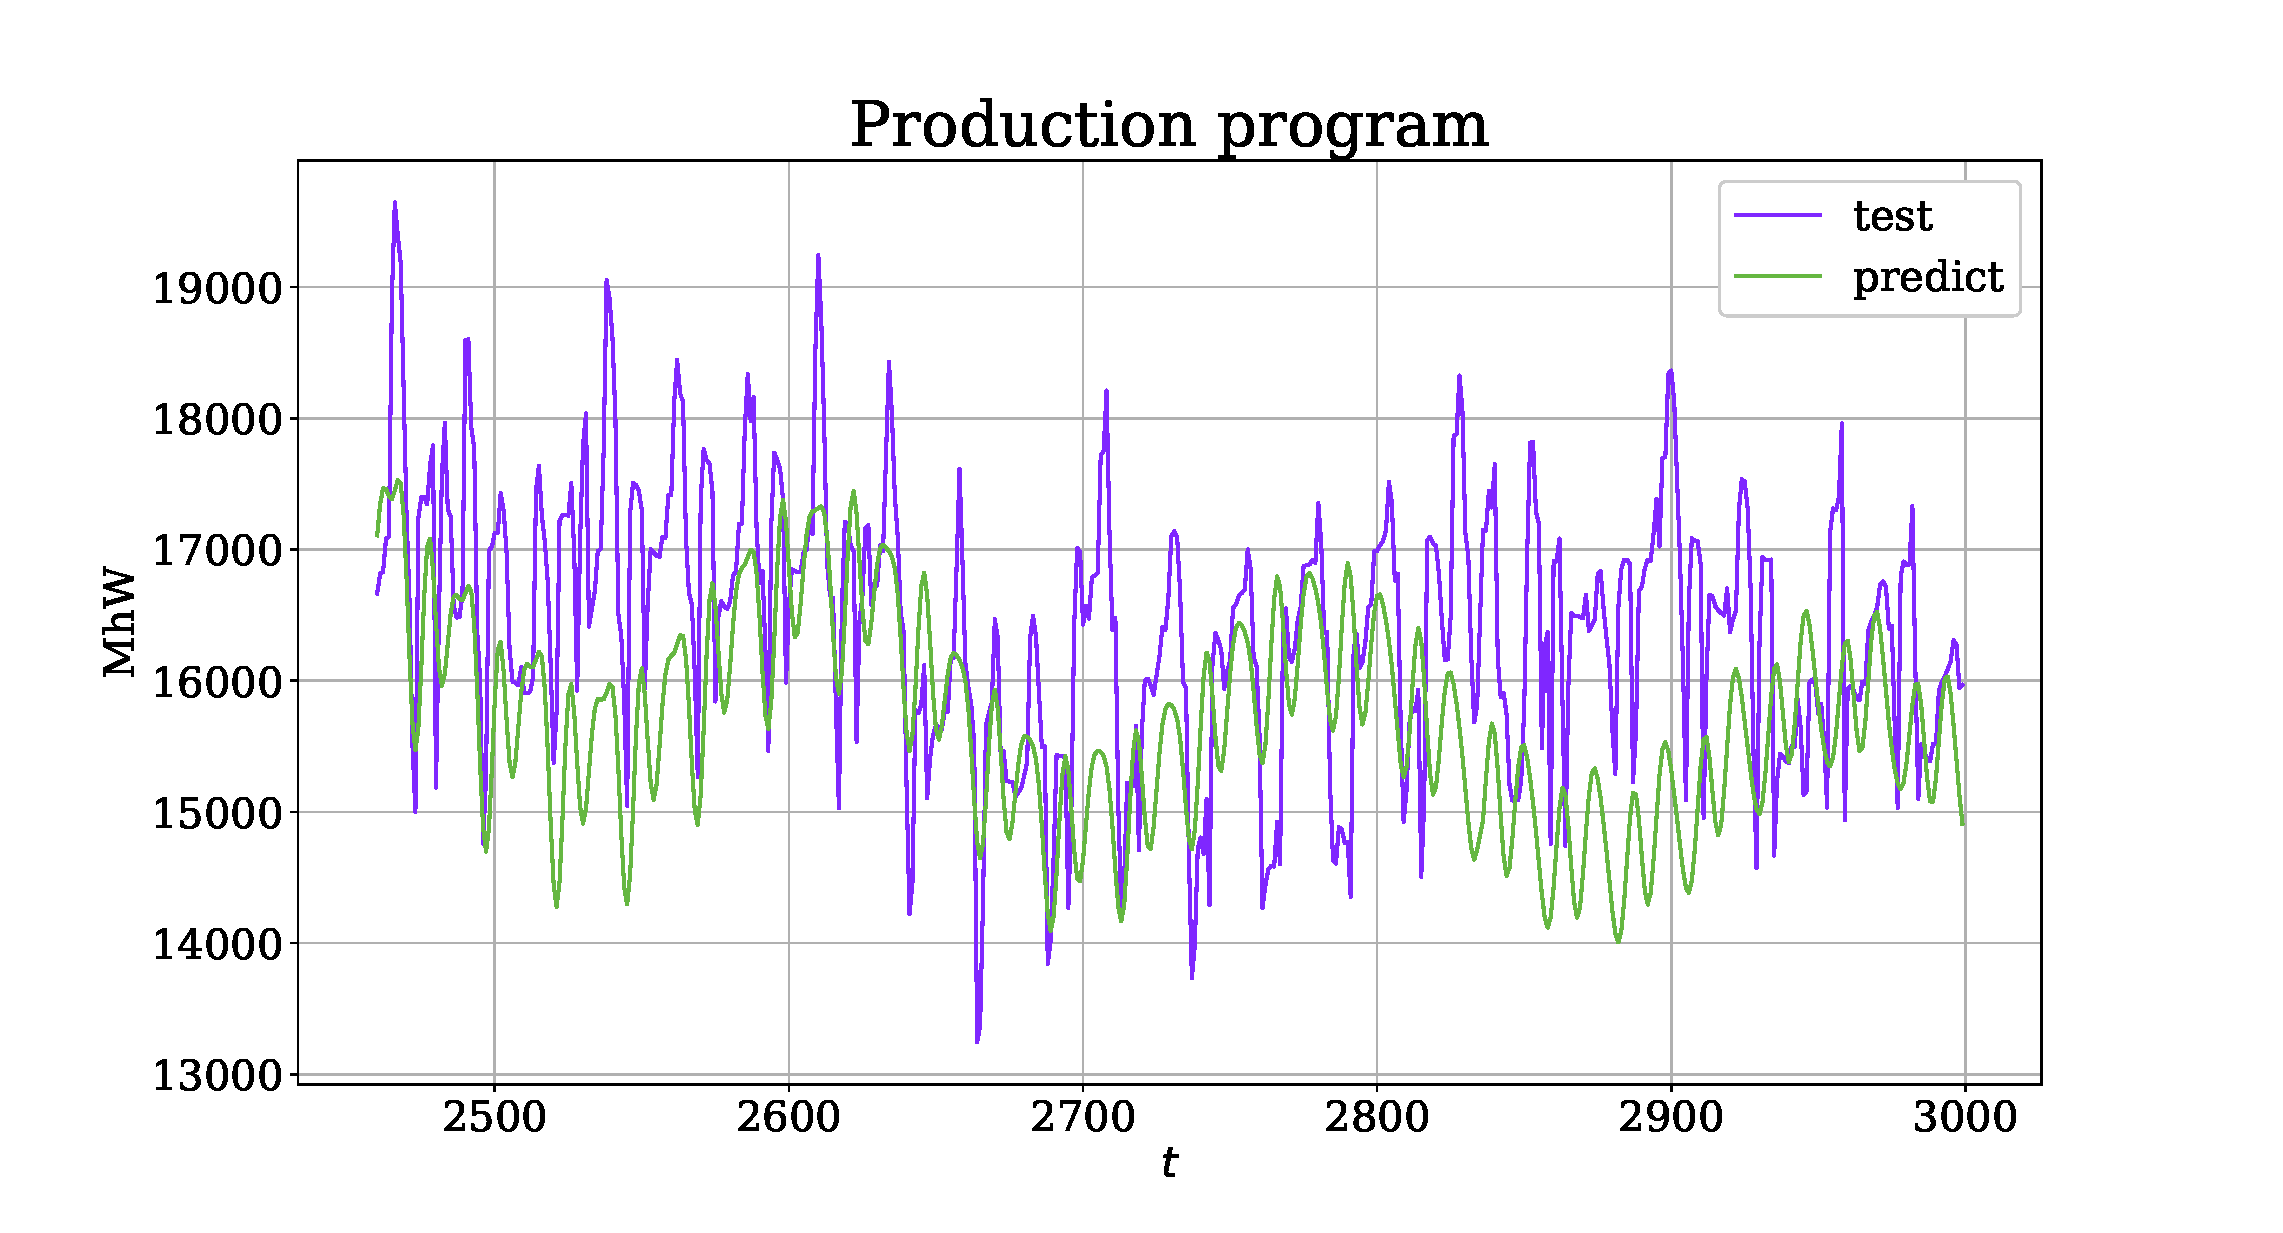
\includegraphics[width=\textwidth, keepaspectratio]{img/electricity/tssa/prediction/Production_program.eps} 
				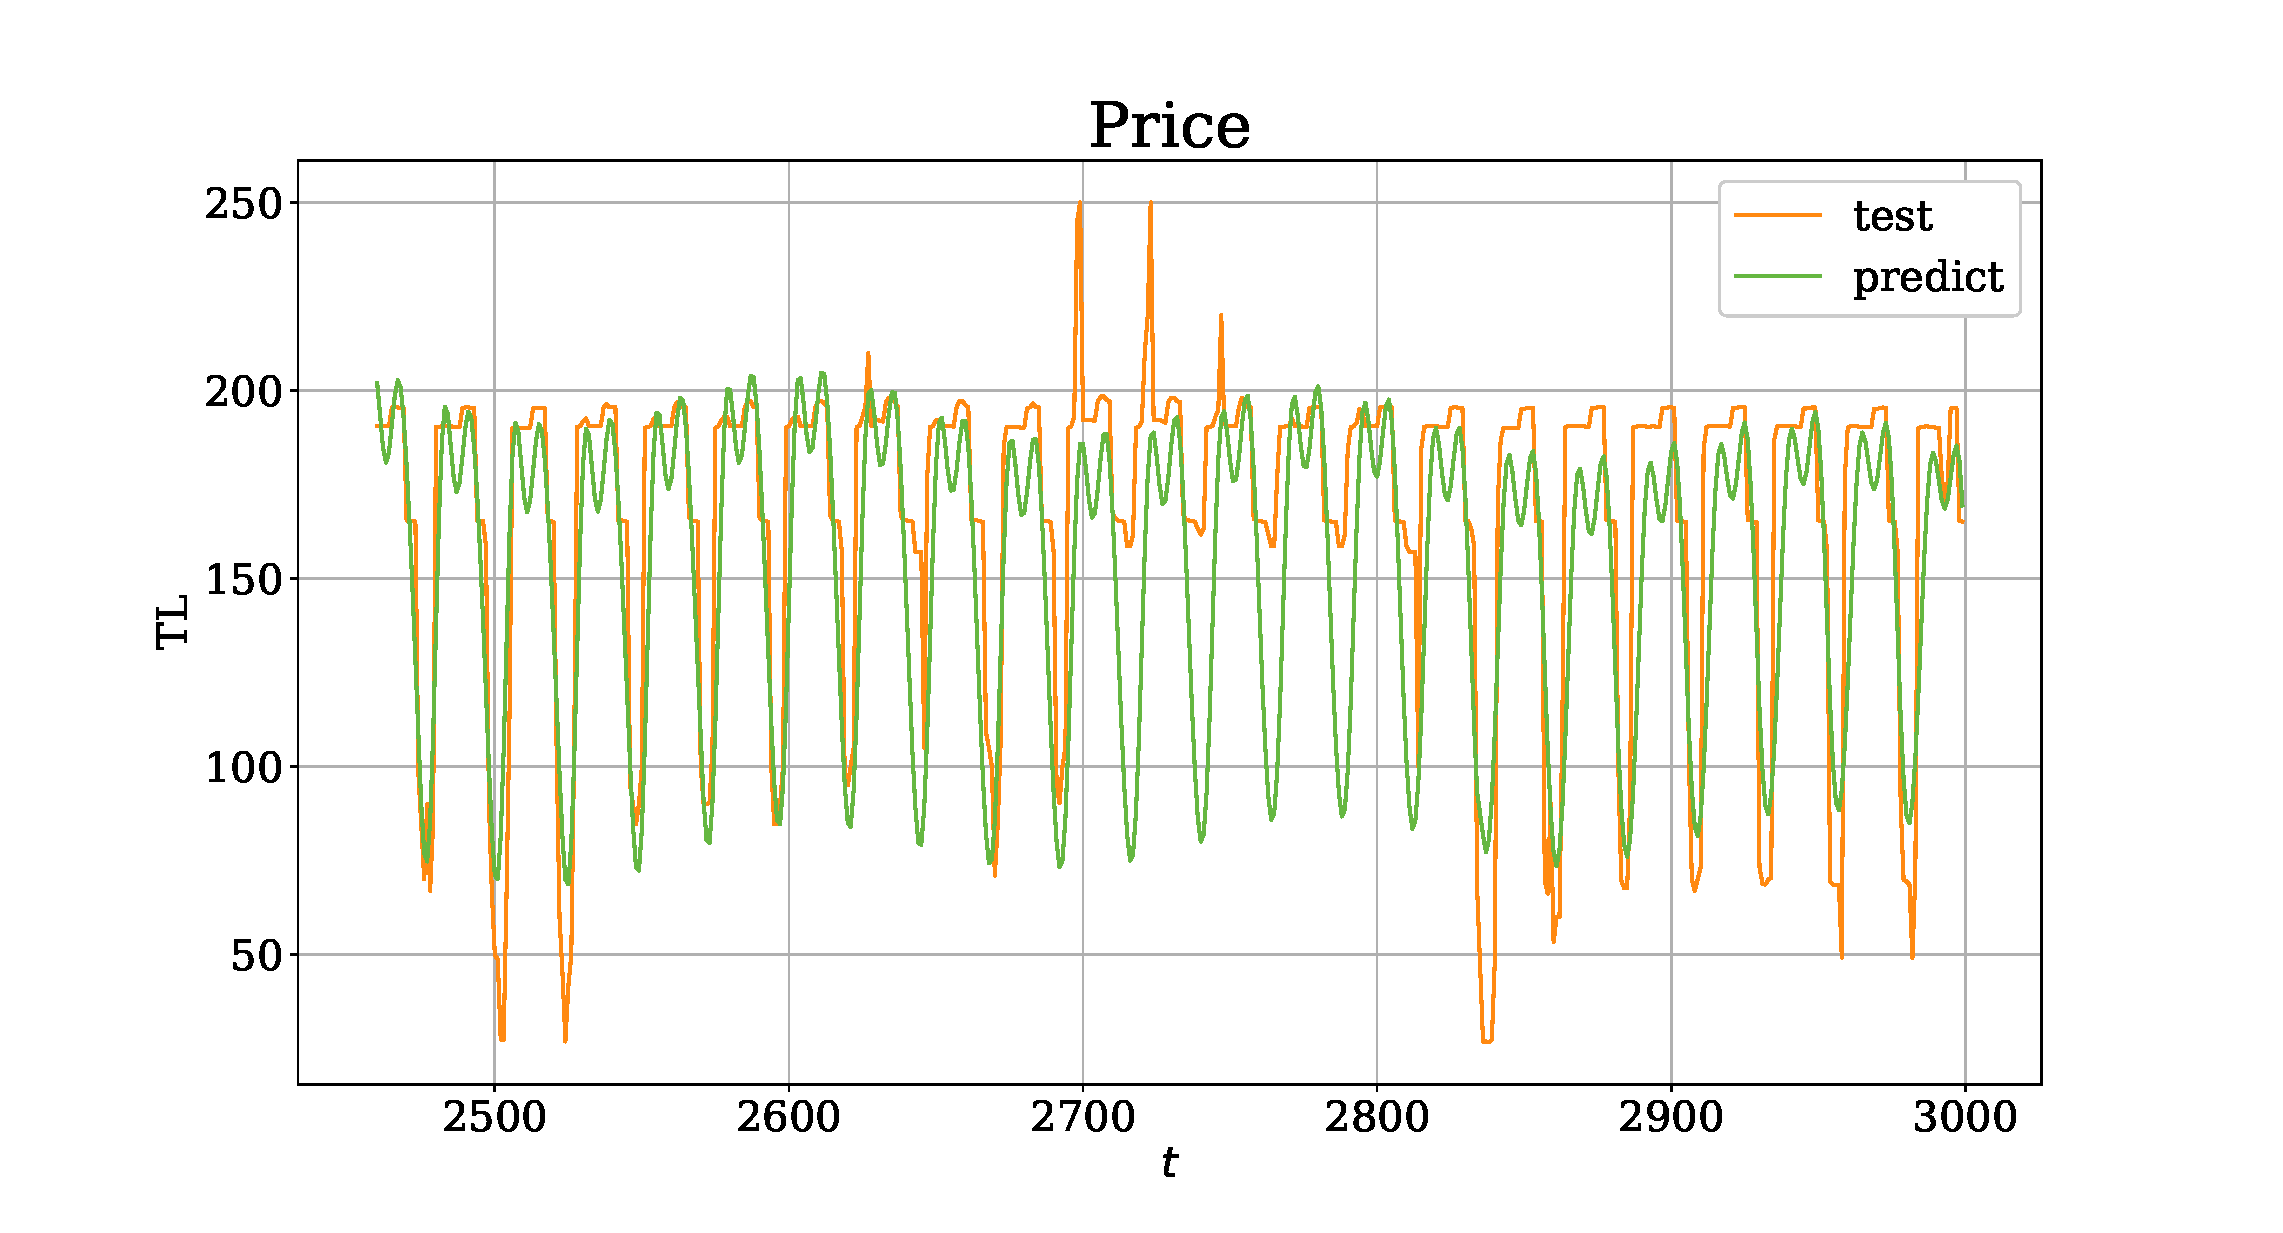
\includegraphics[width=\textwidth, keepaspectratio]{img/electricity/tssa/prediction/Price.eps}    
				\caption{Прогноз tSSA на тестовой части рядов}
				
			\end{figure}
			
			\column{0.5\textwidth}
			
			\begin{figure}[h]
				\centering
				
				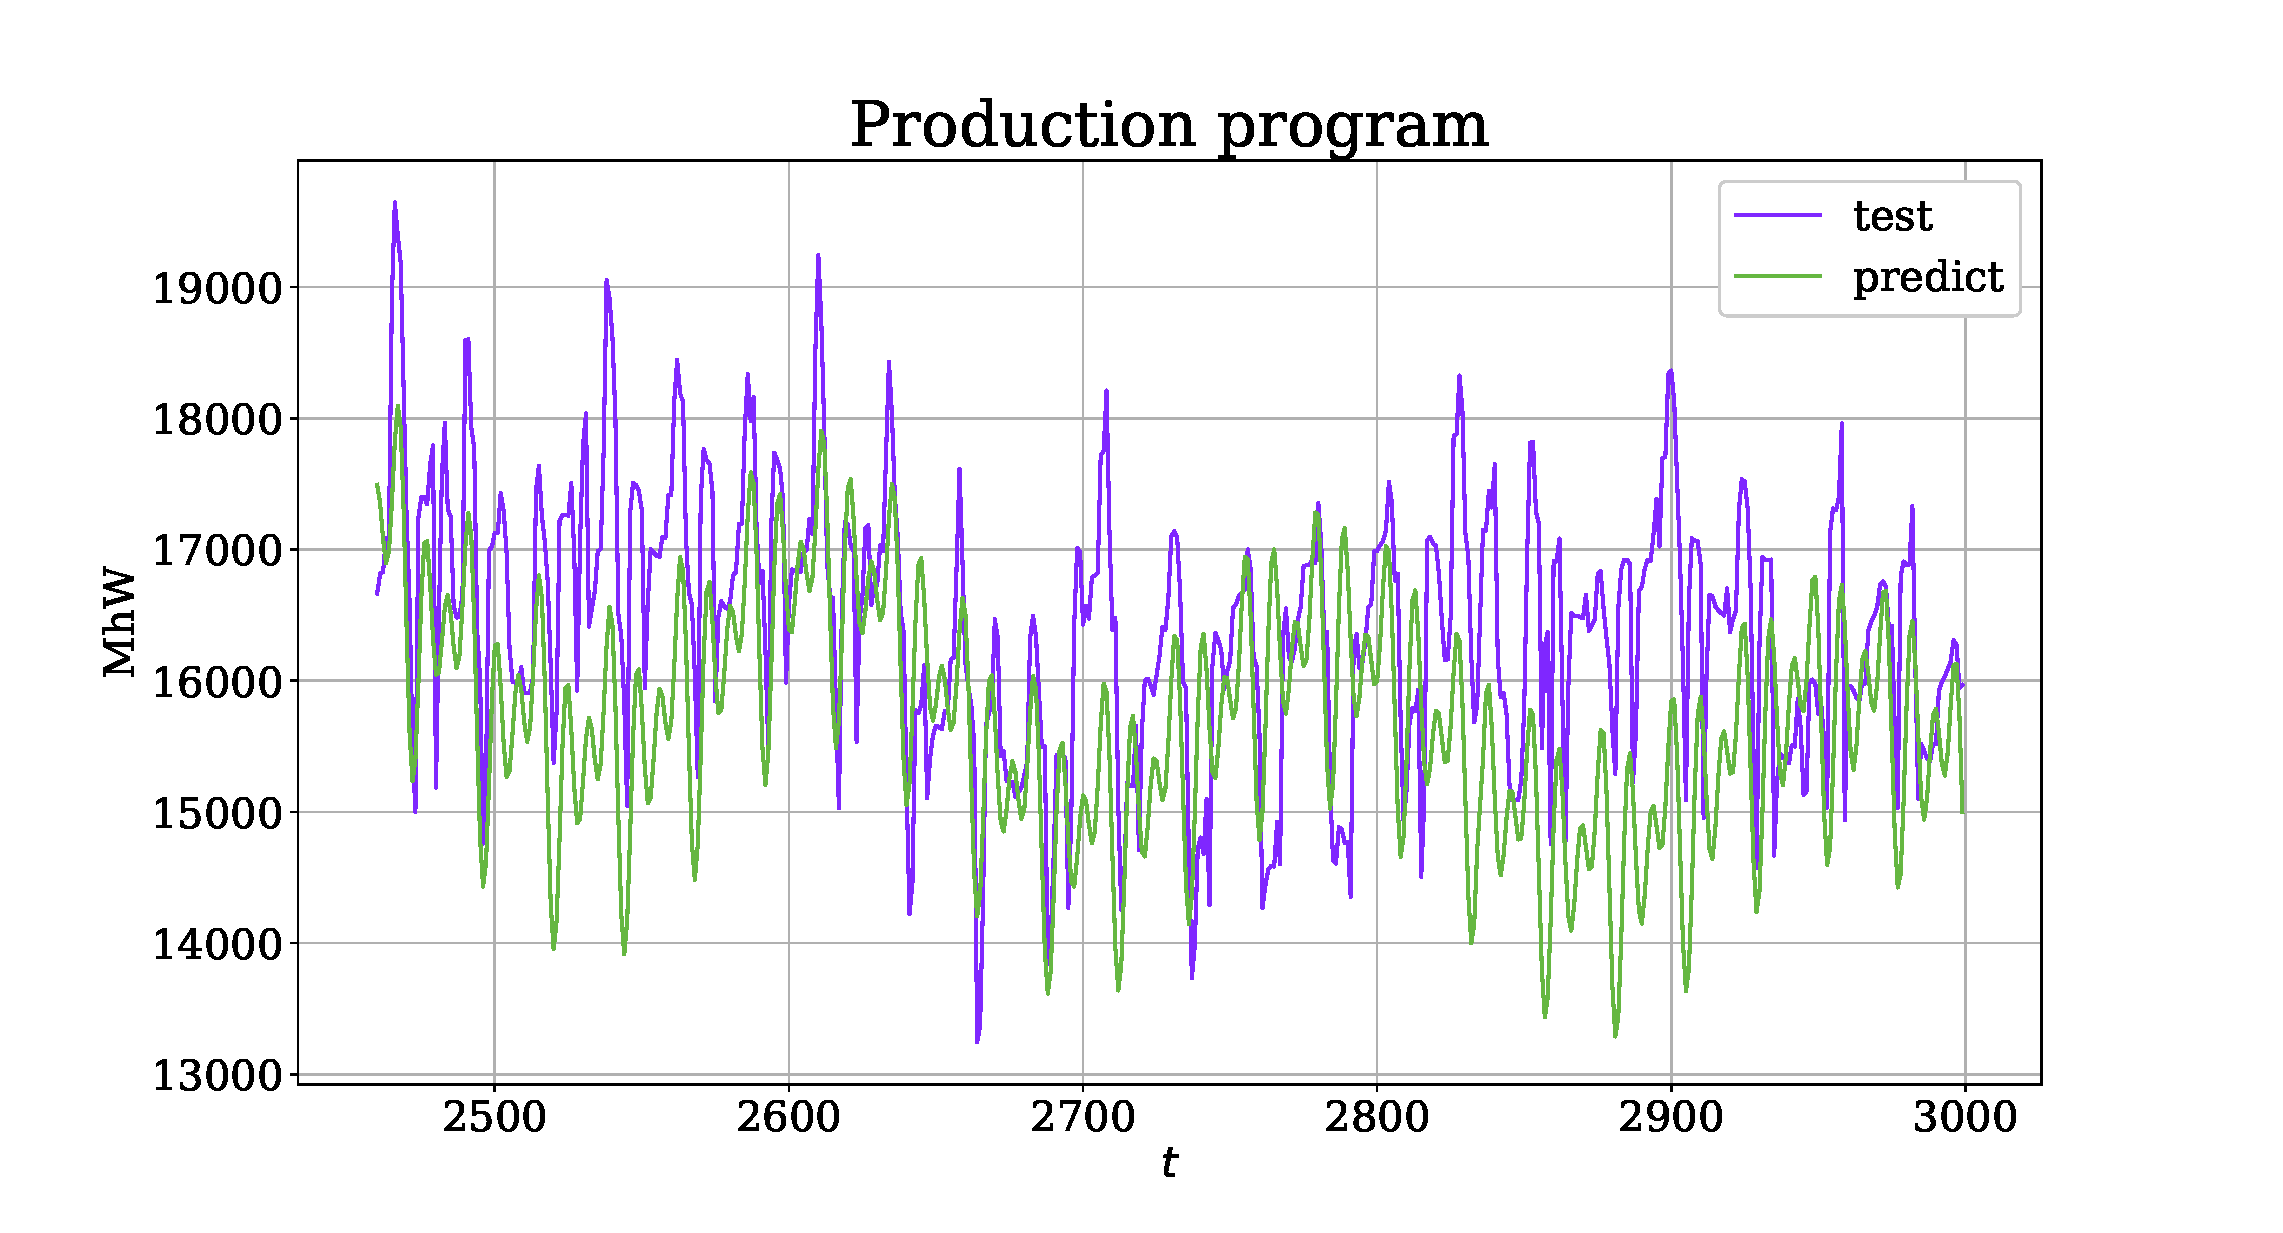
\includegraphics[width=\textwidth, keepaspectratio]{img/electricity/mssa/prediction/Production_program.eps} 
				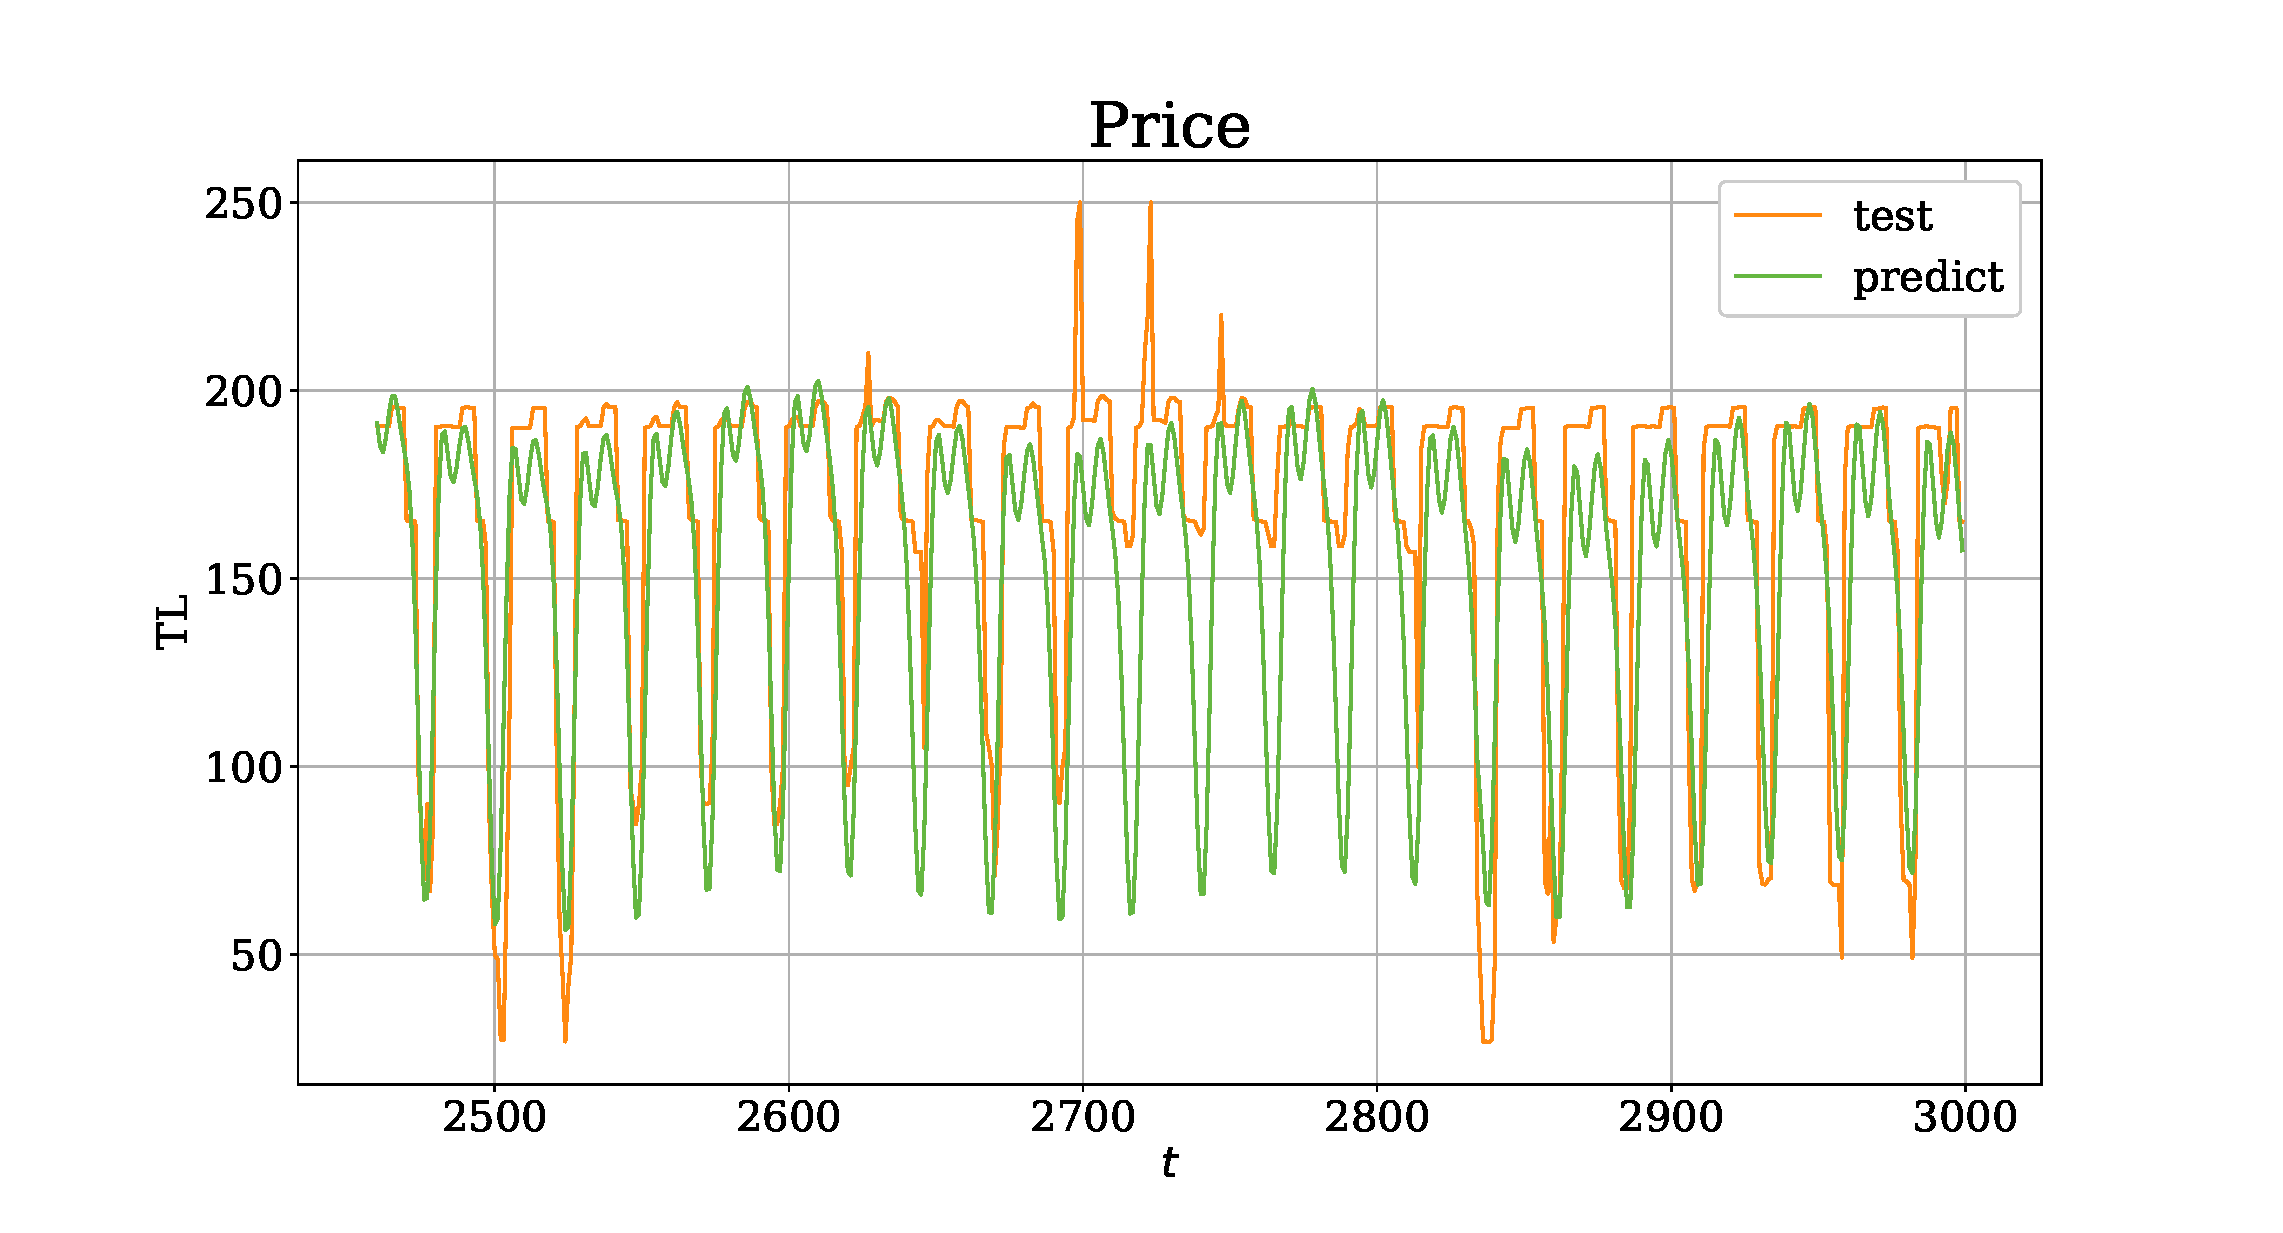
\includegraphics[width=\textwidth, keepaspectratio]{img/electricity/mssa/prediction/Price.eps}    
				\caption{Прогноз mSSA на тестовой части рядов}
				
			\end{figure}
			
		\end{columns}
		
	\end{frame}
	
	\begin{frame}{Электричество. Прогноз}
		
		\begin{columns}
			
			\column{0.5\textwidth}
			
			\begin{figure}[h]
				\centering
				
				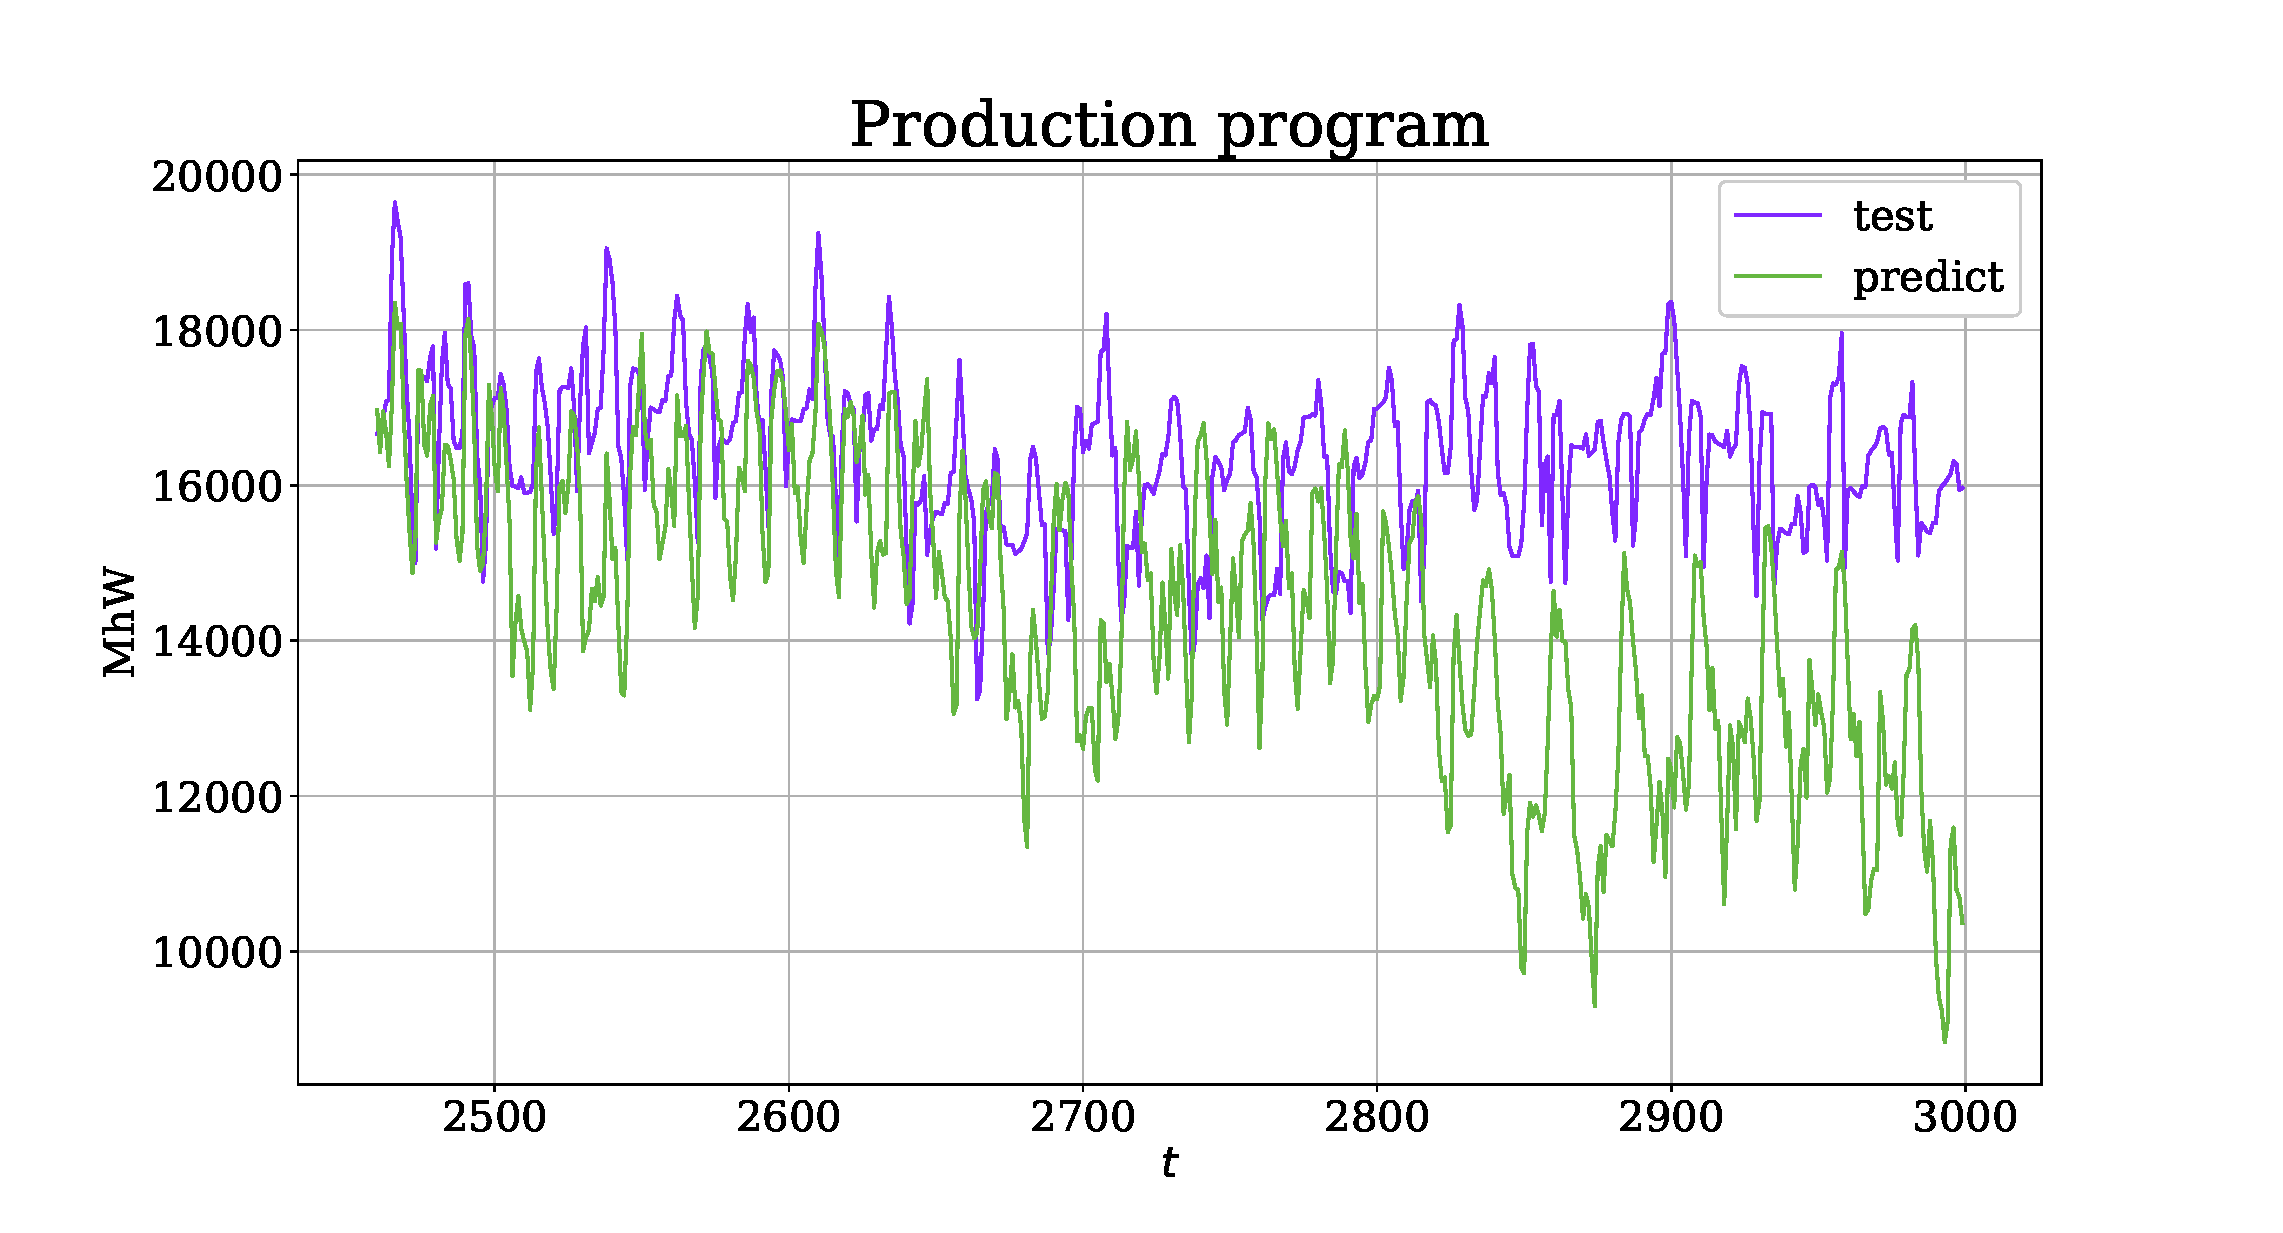
\includegraphics[width=\textwidth, keepaspectratio]{img/electricity/var/prediction/Production_program.eps} 
				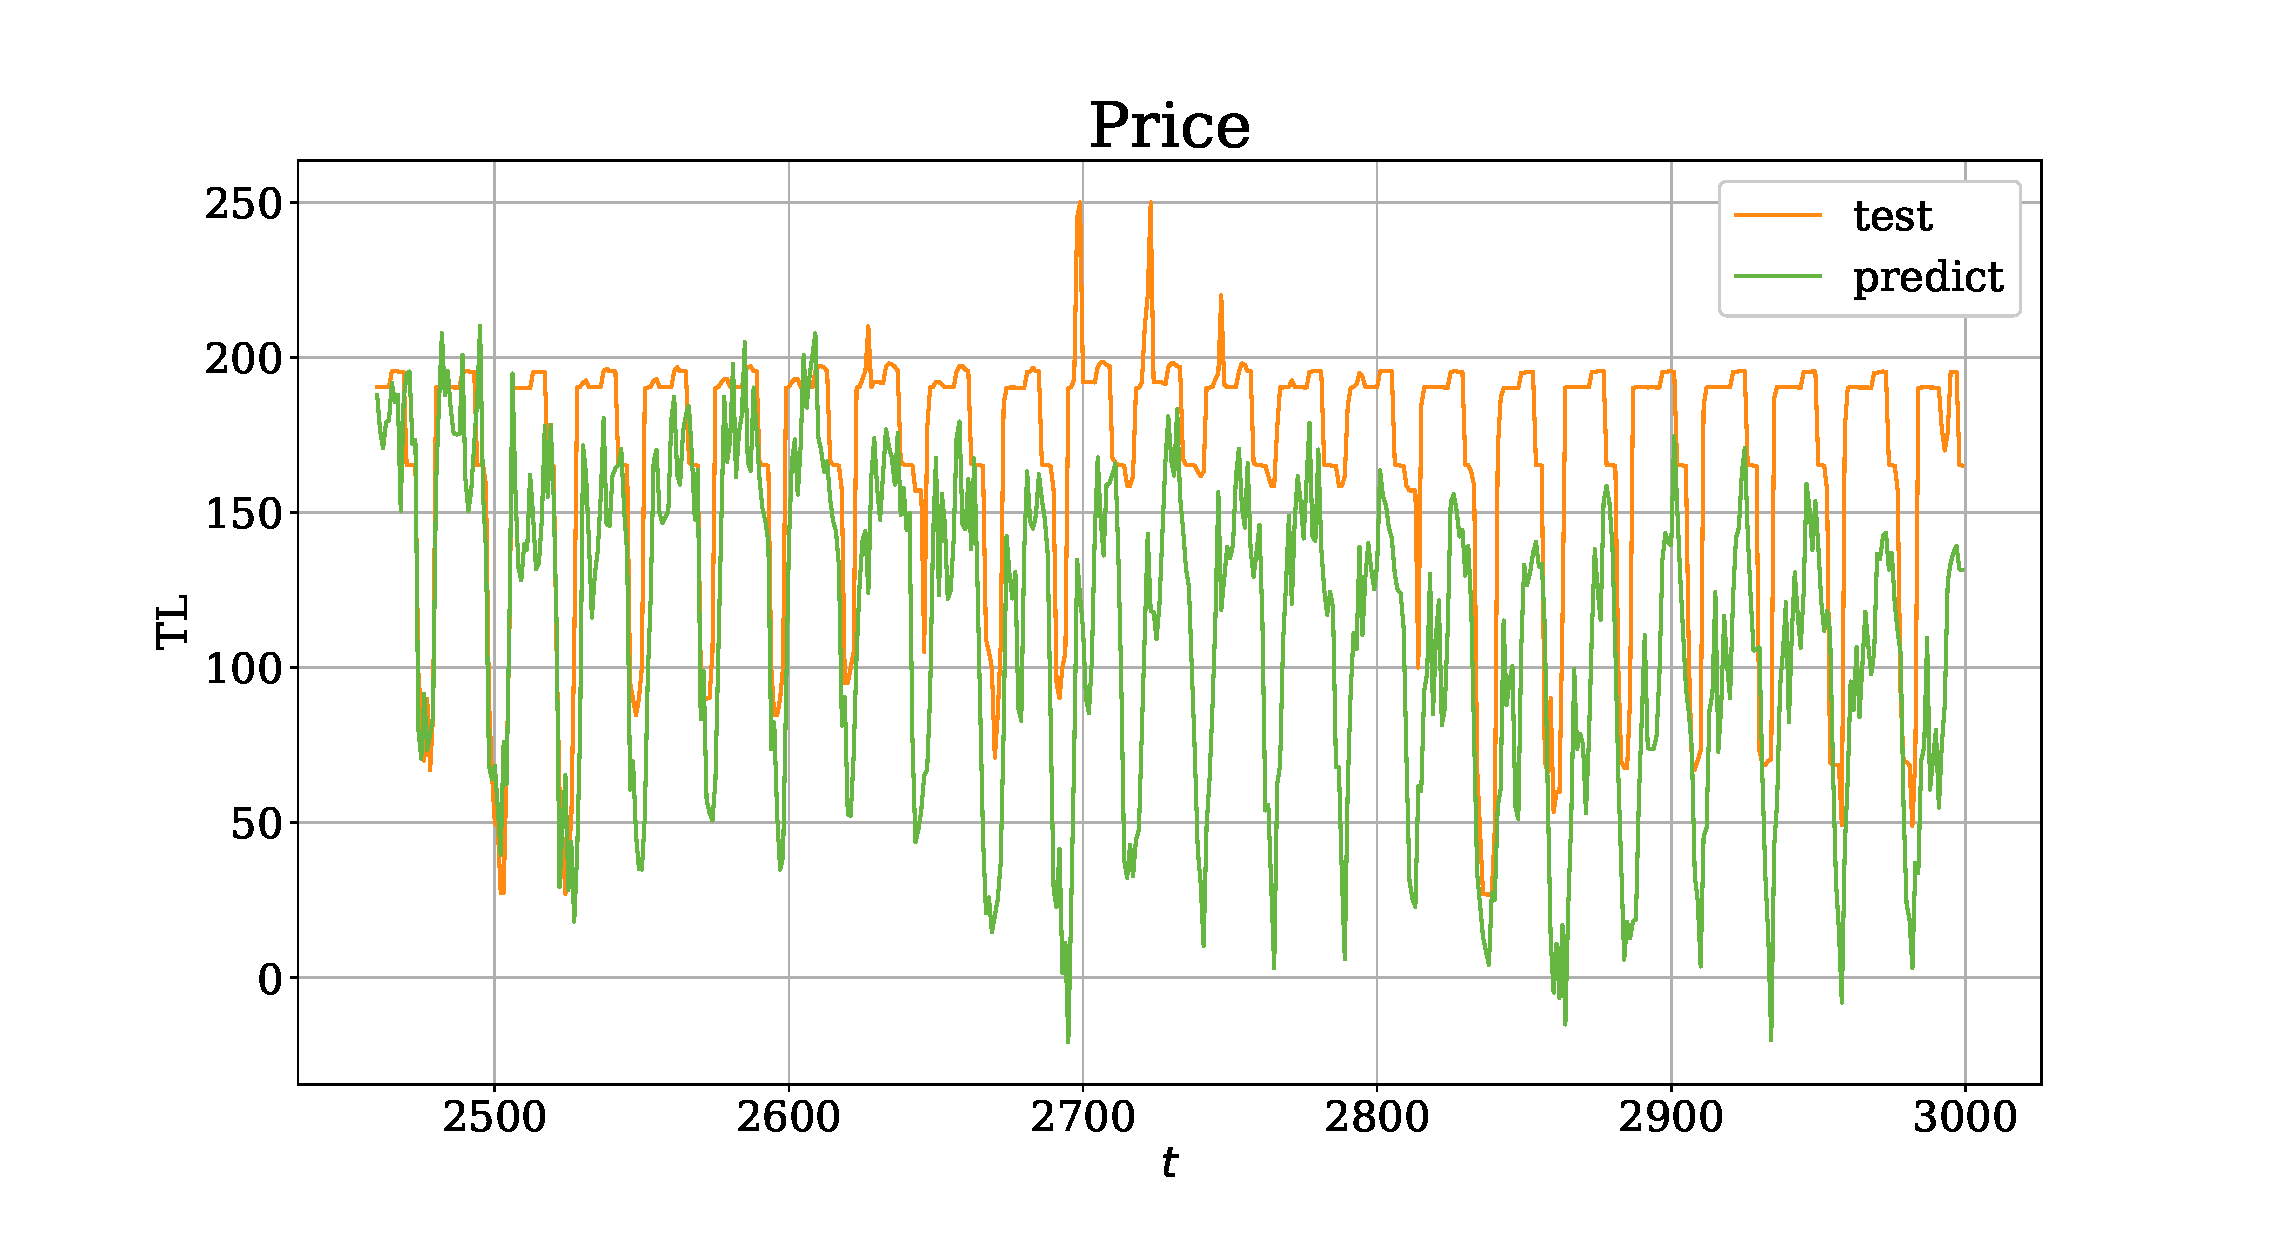
\includegraphics[width=\textwidth, keepaspectratio]{img/electricity/var/prediction/Price.eps}    
				\caption{Прогноз VAR на тестовой части рядов}
				
			\end{figure}
			
			\column{0.5\textwidth}
			
			\begin{figure}[h]
				\centering
				
				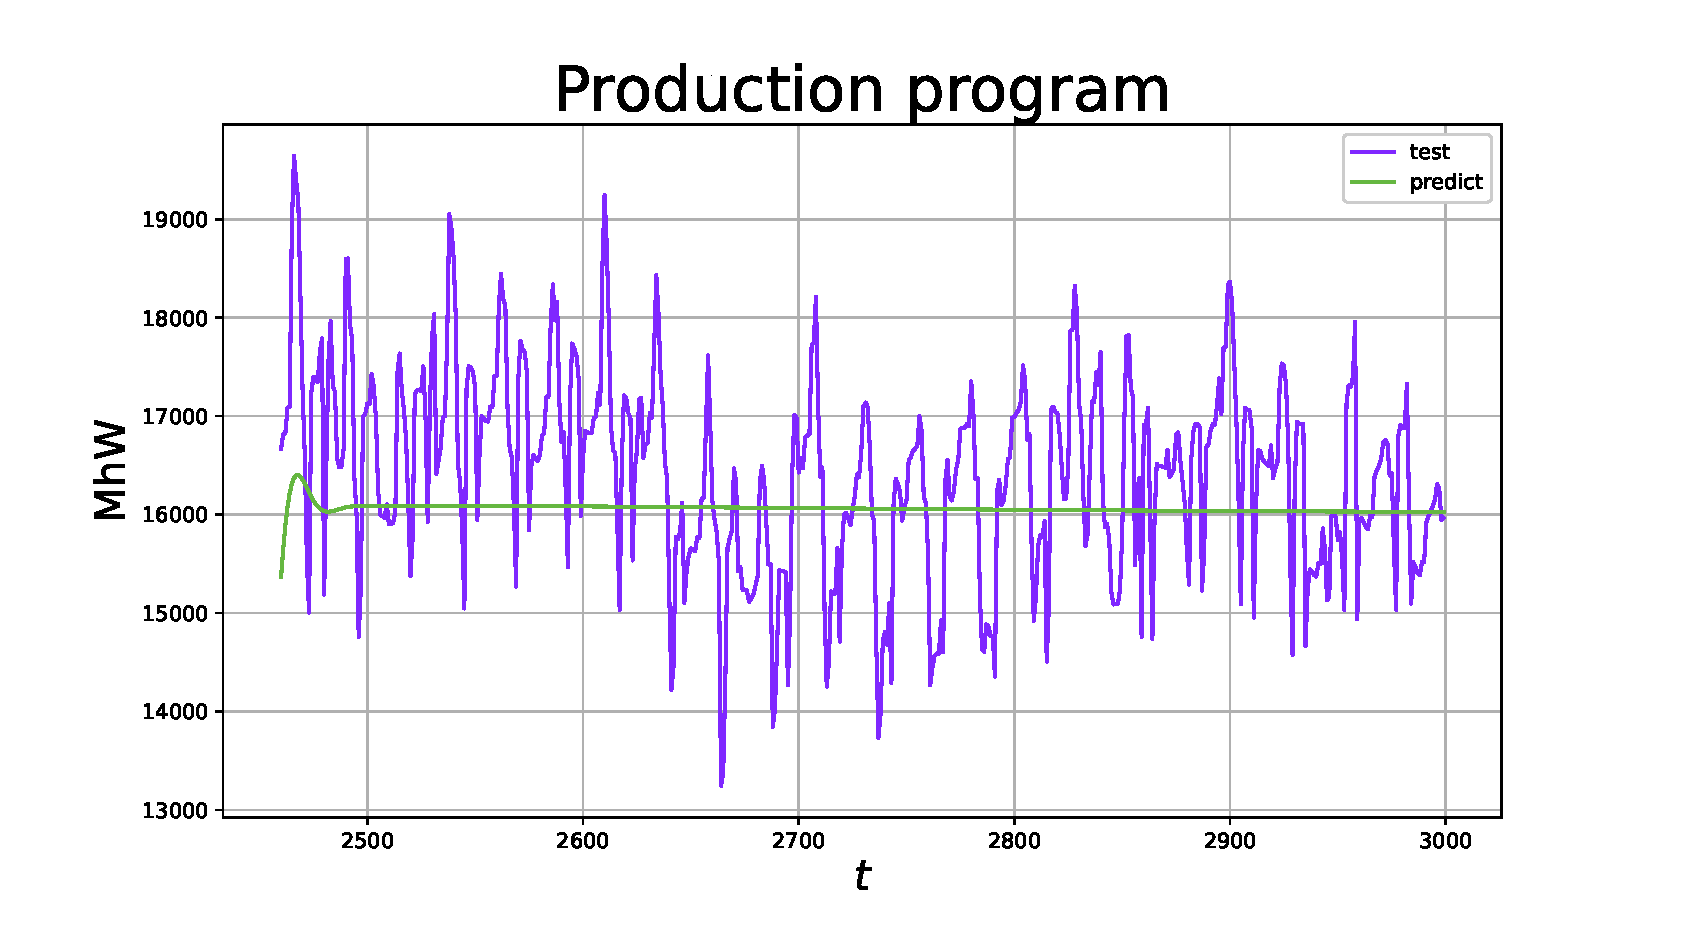
\includegraphics[width=\textwidth, keepaspectratio]{img/electricity/rnn/prediction/Production_program.eps} 
				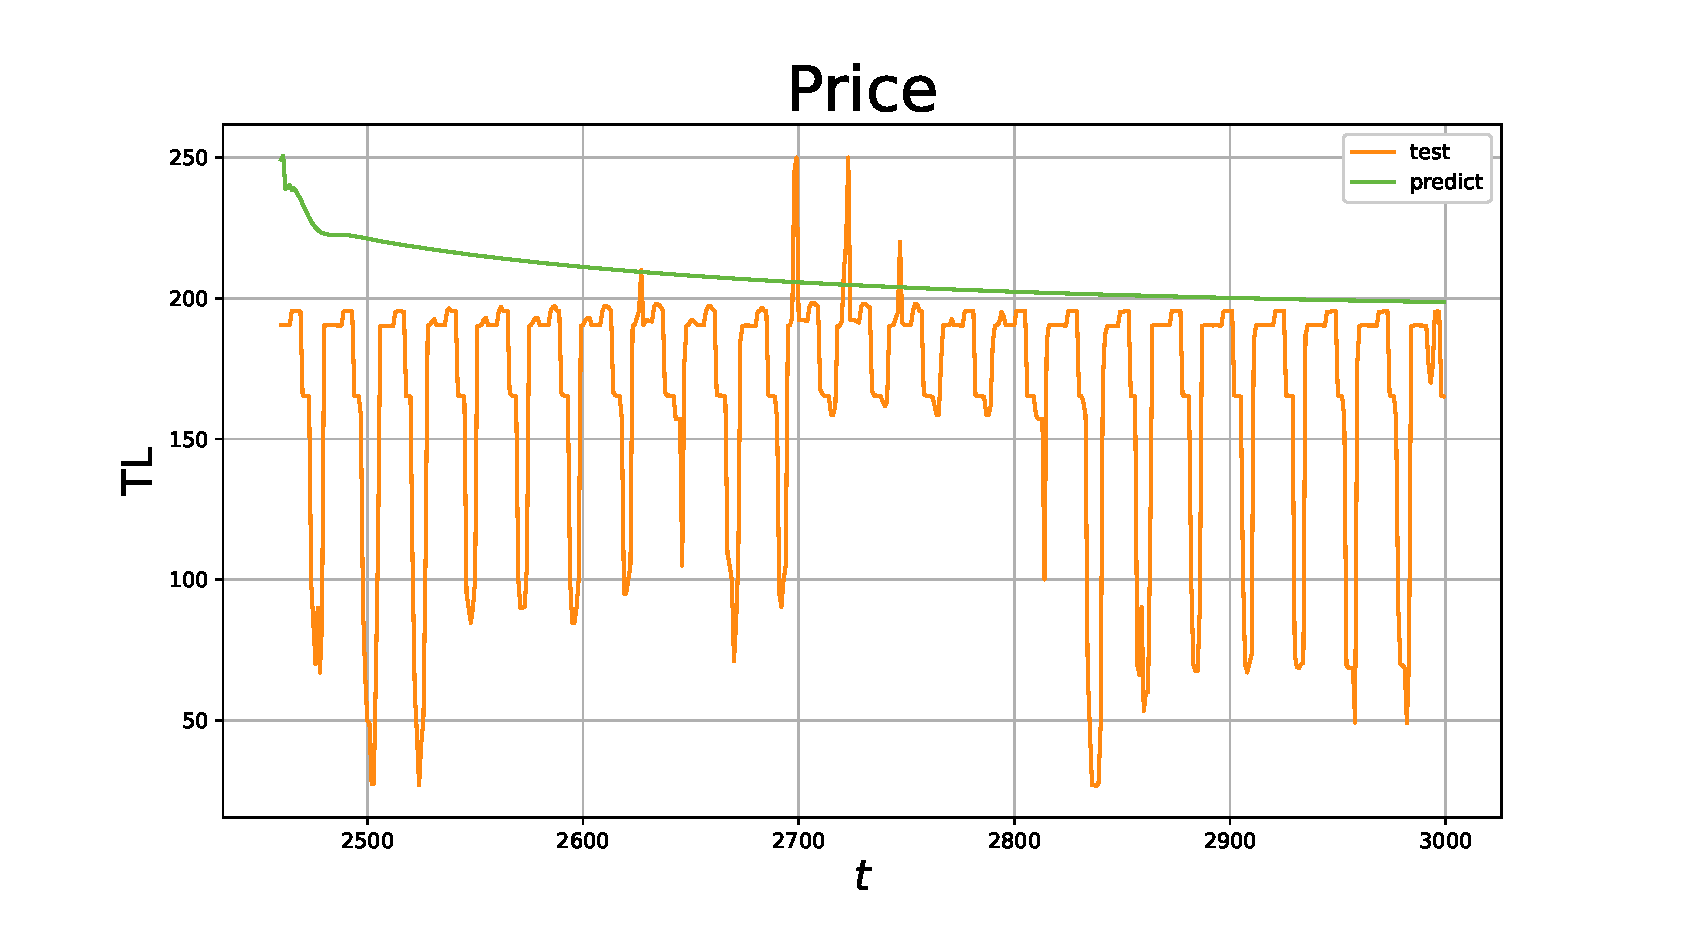
\includegraphics[width=\textwidth, keepaspectratio]{img/electricity/rnn/prediction/Price.eps}    
				\caption{Прогноз RNN на тестовой части рядов}
				
			\end{figure}
			
		\end{columns}
		
	\end{frame}
	
	\begin{frame}{Электричество. Итоги}
		
		\begin{table}[h]
			\caption{Сравнение методов по качеству декомпозиции сигналов.}
			\begin{tabular}{lllll}
				\cline{1-3}
				\multicolumn{1}{|c|}{\textit{Метод}}                        & \multicolumn{1}{c|}{tSSA}  & \multicolumn{1}{c|}{mSSA}  &  &  \\ \cline{1-3}
				\multicolumn{1}{|c|}{\textit{Ср. отн. невязка ганкелизации}} & \multicolumn{1}{c|}{0.802} & \multicolumn{1}{c|}{0.309} &  &  \\ \cline{1-3}
			\end{tabular}
		\end{table}
		
		\begin{table}[h]
			\caption{Сравнение методов по качеству прогноза производства электричества.}
			\begin{tabular}{ccccc}
				\hline
				\multicolumn{1}{|c|}{\textit{Метод}} & \multicolumn{1}{c|}{tSSA} & \multicolumn{1}{c|}{mSSA} & \multicolumn{1}{c|}{VAR} & \multicolumn{1}{c|}{RNN} \\ \hline
				\multicolumn{1}{|c|}{\textit{MSE, $10^6$}}   & \multicolumn{1}{c|}{$1.56$}     & \multicolumn{1}{c|}{$1.50$}     & \multicolumn{1}{c|}{$7.81$}    & \multicolumn{1}{c|}{-}    \\ \hline
				\multicolumn{1}{|c|}{\textit{MAPE}}  & \multicolumn{1}{c|}{$0.059$}     & \multicolumn{1}{c|}{$0.059$}     & \multicolumn{1}{c|}{$0.13$}    & \multicolumn{1}{c|}{-}    \\ \hline
			\end{tabular}
		\end{table}
		
		\begin{table}[h]
			\caption{Сравнение методов по качеству прогноза цены электричества.}
			\begin{tabular}{ccccc}
				\hline
				\multicolumn{1}{|c|}{\textit{Метод}} & \multicolumn{1}{c|}{tSSA} & \multicolumn{1}{c|}{mSSA} & \multicolumn{1}{c|}{VAR} & \multicolumn{1}{c|}{RNN} \\ \hline
				\multicolumn{1}{|c|}{\textit{MSE, $10^3$}}   & \multicolumn{1}{c|}{$1.03$}     & \multicolumn{1}{c|}{$1.03$}     & \multicolumn{1}{c|}{$4.85$}    & \multicolumn{1}{c|}{-}    \\ \hline
				\multicolumn{1}{|c|}{\textit{MAPE}}  & \multicolumn{1}{c|}{$0.18$}     & \multicolumn{1}{c|}{$0.17$}     & \multicolumn{1}{c|}{$0.36$}    & \multicolumn{1}{c|}{-}    \\ \hline   
			\end{tabular}
		\end{table}

	\end{frame}

	
	
\end{document}